%%%%%%%%%%%%%%%%%%%%%%%%%%%%%%%%%%%%%%%%%%%%%%%%%%%%%%%%%%%%%%%%%%%%
%%%%%%%%%%%%%%%%%%%%%%%%%%%%%%%%%%%%%%%%%%%%%%%%%%%%%%%%%%%%%%%%%%%%
%%                                                                %%
%% An example for writting your thesis using LaTeX                %%
%% Original version by Luis Costa,  changes by Perttu Puska       %%
%% Support for Swedish added 15092014                             %%
%%                                                                %%
%% Esimerkki opinnäytteen tekemisestä LaTeX:lla                   %%
%% Alkuperäinen versio Luis Costa,  muutokset Perttu Puska        %%
%% Ruotsinkielen tuki lisätty 05032014                            %%
%%                                                                %%
%% This example consists of the files                             %%
%% Tähän esimerkkiin kuuluu tiedostot                             %%
%%         thesistemplate.tex (versio 2.0)                        %%
%%         opinnaytepohja.tex (versio 2.0) (for text in Finnish)  %%
%%         aaltothesis.cls (versio 2.0)                           %%
%%         kuva1.eps                                              %%
%%         kuva2.eps                                              %%
%%         kuva1.pdf                                              %%
%%         kuva2.pdf                                              %%
%%                                                                %%
%%                                                                %%
%% Typeset either with                                            %%
%% Kääntäminen joko                                               %%
%% latex:                                                         %%
%%             $ latex opinnaytepohja                             %%
%%             $ latex opinnaytepohja                             %%
%%                                                                %%
%%   Result is the file opinnayte.dvi, which                      %%
%%   is converted to ps format as follows:                        %%
%%   Tuloksena on tiedosto opinnayte.dvi, joka                    %%
%%   muutetaan ps-muotoon seuraavasti                             %%
%%                                                                %%
%%             $ dvips opinnaytepohja -o                          %%
%%                                                                %%
%%   and then to pdf as follows:                                  %%
%%   ja edelleen pdf-muotoon seuraavasti                          %%
%%                                                                %%
%%             $ ps2pdf opinnaytepohja.ps                         %%
%%                                                                %%
%% Or                                                             %%
%% Tai                                                            %%
%% pdflatex:                                                      %%
%%             $ pdflatex opinnaytepohja                          %%
%%             $ pdflatex opinnaytepohja                          %%
%%                                                                %%
%%   Result is the file opinnaytepohja.pdf                        %%
%%   Tuloksena on tiedosto opinnaytepohja.pdf                     %%
%%                                                                %%
%% Explanatory comments in this example begin with                %%
%% the characters %%, and changes that the user can make          %%
%% with the character %                                           %%
%% Selittävät kommentit on tässä esimerkissä varustettu           %%
%% %%-merkeillä ja muutokset, joita käyttäjä voi tehdä,           %%
%% on varustettu %-merkeillä                                      %%
%%                                                                %%
%%%%%%%%%%%%%%%%%%%%%%%%%%%%%%%%%%%%%%%%%%%%%%%%%%%%%%%%%%%%%%%%%%%%
%%%%%%%%%%%%%%%%%%%%%%%%%%%%%%%%%%%%%%%%%%%%%%%%%%%%%%%%%%%%%%%%%%%%

%% Uncomment one of these, if you write in English:
%% the 1st when using pdflatex, which directly typesets your document in
%% pdf (use jpg or pdf figures), or
%% the 2nd when producing a ps file (use eps figures, don't use ps figures!).
\documentclass[english,12pt,a4paper,pdftex,elec,utf8]{aaltothesis}
%\documentclass[english,12pt,a4paper,dvips]{aaltothesis}

%% To the \documentclass above
%% specify your school: arts, biz, chem, elec, eng, sci
%% specify the character encoding scheme used by your editor: utf8, latin1

%%
%% Käytä toinen näistä, jos kirjoitat suomeksi:
%% ensimmäinen, jos käytät pdflatexia, joka kääntää tekstin suoraan
%% pdf-tiedostoksi (kuvat on oltava jpg- tai pdf-tiedostoina)
%% toinen, jos haluat tuottaa ps-tiedostoa (käytä eps-formaattia kuville,
%% alä käytä ps-muotoisia kuvia!)
%%
%% Use one of these if you write in Finnish:
%%
%\documentclass[finnish,12pt,a4paper,pdftex,elec,utf8]{aaltothesis}
%\documentclass[finnish,12pt,a4paper,dvips]{aaltothesis}

%% Kirjoita y.o. \documentclass optioiksi
%% korkeakoulusi näistä: arts, biz, chem, elec, eng, sci
%% editorisi käyttämä merkkikoodaustapa: utf8, latin1
%%

\usepackage{graphicx}

%% Use this if you write hard core mathematics, these are usually needed
%%
%% Matematiikan fontteja, symboleja ja muotoiluja lisää, näitä tarvitaan usein
\usepackage{amsfonts,amssymb,amsbsy,amsmath}
\usepackage{epigraph}
\usepackage{commath}
\usepackage{listings}
\usepackage{bm}
%% Use the macros in this package to change how the hyperref package below
%% typesets its hypertext -- hyperlink colour, font, etc. See the package
%% documentation. It also defines the \url macro, so use the package when
%% not using the hyperref package.
%%
%% Jos et jostain syystä pidä, miten alla oleva hyperref-paketti käyttää
%% fontteja, värejä yms., käytä tämän paketin makroja muuttamaan
%% fonttimäärittelyt. Katso paketin dokumentaatiota. Paketti määrittelee
%% \url-makron, joten ota paketti käyttöön, jos et käytä hyperref-pakettia.
%\usepackage{url}

%% Use this if you want to get links and nice output. Works well with pdflatex.
%%
%% Saat pdf-tiedoston viittaukset ja linkit kuntoon seuraavalla paketilla.
%% Paketti toimii erityisen hyvin pdflatexin kanssa.
\usepackage{hyperref}
\hypersetup{pdfpagemode=UseNone, pdfstartview=FitH,
  colorlinks=true,urlcolor=red,linkcolor=blue,citecolor=black,
  pdftitle={Default Title, Modify},pdfauthor={Samuli Ulmanen},
  pdfkeywords={Modify keywords}}


%% All that is printed on paper starts here
%%
%% Kaikki mikä paperille tulostuu, on tämän jälkeen
\begin{document}

%% Change the school field to specify your school if the automatically
%% set name is wrong
%%
%% Korjaa vastaamaan korkeakouluasi, jos automaattisesti asetettu nimi on
%% virheellinen
% \university{aalto-yliopisto}
% \university{aalto University}
% \school{Sähkötekniikan korkeakoulu}
% \school{School of Electrical Engineering}

%% Only for B.Sc. thesis: Choose your degree programme.
%%
%% Vain kandityölle: Korjaa seuraavat vastaamaan koulutusohjelmaasi
\degreeprogram{Electronics and electrical engineering}
%\degreeprogram{Elektroniikka ja sähkötekniikka}
%%

%% ONLY FOR M.Sc. AND LICENTIATE THESIS: Specify your department,
%% professorship and professorship code.
%%
%% Vain DI/M.Sc.- ja lisensiaatintyölle: valitse laitos,
%% professuuri ja sen professuurikoodi.
\department{Department of Radio Science and Technology}
%\department{Radiotieteen ja -tekniikan laitos}

\professorship{Circuit theory}
%\professorship{Piiriteoria}
\code{S-55}
%%

%% Valitse yksi näistä kolmesta
%%
%% Choose one of these:
%\univdegree{BSc}
\univdegree{MSc}
%\univdegree{Lic}

%% Oma nimi
%%
%% Should be self explanatory...
\author{Teemu Teekkari}

%% Your thesis title comes here and again before a possible abstract in
%% Finnish or Swedish . If the title is very long and latex does an
%% unsatisfactory job of breaking the lines, you will have to force a
%% linebreak with the \\ control character.
%% Do not hyphenate titles.
%%
%% Opinnäytteen otsikko tulee tähän ja uudelleen englannin- tai
%% ruostinkielisen abstraktin yhteydessä. Älä tavuta otsikkoa ja
%% vältä liian pitkää otsikkotekstiä. Jos latex ryhmittelee otsikon
%% huonosti, voit joutua pakottamaan rivinvaihdon \\ kontrollimerkillä.
%% Muista että otsikkoja ei tavuteta!
%% Jos otsikossa on ja-sana, se ei jää rivin viimeiseksi sanaksi
%% vaan aloittaa uuden rivin.
\thesistitle{Thesis template}

\place{Espoo}

%% For B.Sc. thesis use the date when you present your thesis.
%%
%% Kandidaatintyön päivämäärä on sen esityspäivämäärä!
\date{28.2.2014}

%% B.Sc. or M.Sc. thesis supervisor
%% Note the "\" after the comma. This forces the following space to be
%% a normal interword space, not the space that starts a new sentence.
%% This is done because the fullstop isn't the end of the sentence that
%% should be followed by a slightly longer space but is to be followed
%% by a regular space.
%%
%% Kandidaattiseminaarin vastuuopettaja tai diplomityön valvoja.
%% Huomaa tittelissä "\" -merkki pisteen jälkeen,
%% ennen välilyöntiä ja seuraavaa merkkijonoa.
%% Näin tehdään, koska kyseessä ei ole lauseen loppu, jonka jälkeen tulee
%% hieman pidempi väli vaan halutaan tavallinen väli.
\supervisor{Prof.\ Pirjo Professori} %{Prof.\ Pirjo Professori}

%% B.Sc. or M.Sc. thesis advisors(s). You can give upto two advisors in
%% this template. Check with your supervisor how many official advisors
%% you can have.
%%
%% Kandidaatintyön ohjaaja(t) tai diplomityön ohjaaja(t). Ohjaajia saa
%% olla korkeintaan kaksi.
%%
%\advisor{Prof.\ Pirjo Professori}
\advisor{Lic.Sc.\ (Tech.) Janne Jalkanen}
%\advisor{M.Sc.\ Polli Pohjaaja}

%% Aalto logo: syntax:
%% Aaltologo: syntaksi:
%%
%% \uselogo{aaltoRed|aaltoBlue|aaltoYellow|aaltoGray|aaltoGrayScale}{?|!|''}
%%
%% Logo language is set to be the same as the document language.
%% Logon kieli on sama kuin dokumentin kieli
%%
\uselogo{aaltoRed}{''}

%% Create the coverpage
%%
%% Tehdään kansilehti
\makecoverpage


%% Note that when writting your master's thesis in English, place
%% the English abstract first followed by the possible Finnish abstract

%% English abstract.
%% All the information required in the abstract (your name, thesis title, etc.)
%% is used as specified above.
%% Specify keywords
%%
%% Kaikki tiivistelmässä tarvittava tieto (nimesi, työnnimi, jne.) käytetään
%% niin kuin se on yllä määritelty.
%% Avainsanat
%%
\keywords{For keywords choose concepts that are central to your thesis}
%% Abstract text
\begin{abstractpage}[english]
  Your abstract in English. Try to keep the abstract short; approximately
  100 words should be enough. The abstract explains your research topic,
  the methods you have used, and the results you obtained.
  Your abstract in English. Try to keep the abstract short; approximately
  100 words should be enough. The abstract explains your research topic,
  the methods you have used, and the results you obtained.

  Your abstract in English. Try to keep the abstract short; approximately
  100 words should be enough. The abstract explains your research topic,
  the methods you have used, and the results you obtained.
  Your abstract in English. Try to keep the abstract short; approximately
  100 words should be enough. The abstract explains your research topic,
  the methods you have used, and the results you obtained.
\end{abstractpage}

%% Force a new page so that the possible English abstract starts on a new page
%%
%% Pakotetaan uusi sivu varmuuden vuoksi, jotta
%% mahdollinen suomenkielinen ja englanninkielinen tiivistelmä
%% eivät tule vahingossakaan samalle sivulle
\newpage
%
%% Abstract in Finnish.  Delete if you don't need it.
%%
%% Suomenkielinen tiivistelmä. Poista, jos et tarvitse sitä.
%% Opinnäytteen ostikko suomeksi
\thesistitle{Opinnäyteohje}
\advisor{TkT Olli Ohjaaja}
\degreeprogram{Electronics and electrical engineering}
\department{Radiotieteen ja -tekniikan laitos}
\professorship{Piiriteoria}
%% Avainsanat
\keywords{Vastus, Resistanssi,\\ Lämpötila}
%% Tiivistelmän tekstiosa
\begin{abstractpage}[finnish]
  Tiivistelmässä on lyhyt selvitys (noin 100 sanaa)
  kirjoituksen tärkeimmästä sisällöstä: mitä ja miten on tutkittu,
  sekä mitä tuloksia on saatu.
  Tiivistelmässä on lyhyt selvitys (noin 100 sanaa)
  kirjoituksen tärkeimmästä sisällöstä: mitä ja miten on tutkittu,
  sekä mitä tuloksia on saatu.

  Tiivistelmässä on lyhyt selvitys (noin 100 sanaa)
  kirjoituksen tärkeimmästä sisällöstä: mitä ja miten on tutkittu,
  sekä mitä tuloksia on saatu.
  Tiivistelmässä on lyhyt selvitys (noin 100 sanaa)
  kirjoituksen tärkeimmästä sisällöstä: mitä ja miten on tutkittu,
  sekä mitä tuloksia on saatu.
  Tiivistelmässä on lyhyt selvitys (noin 100 sanaa)
  kirjoituksen tärkeimmästä sisällöstä: mitä ja miten on tutkittu,
  sekä mitä tuloksia on saatu.
\end{abstractpage}

%% Force new page so that the Swedish abstract starts from a new page
\newpage
%
%% Swedish abstract. Delete if you don't need it.
%%
\thesistitle{Arbetets titel}
\advisor{TkD Olli Ohjaaja} %
\degreeprogram{Electronik och electroteknik}
\department{Institutionen för radiovetenskap och -teknik}%
\professorship{Kretsteori}  %
%% Abstract keywords
\keywords{Nyckelord p\aa{} svenska,\\ Temperatur}
%% Abstract text
\begin{abstractpage}[swedish]
 Sammandrag p\aa{} svenska.
 Try to keep the abstract short, approximately
 100 words should be enough. Abstract explains your research topic,
 the methods you have used, and the results you obtained.
\end{abstractpage}

%% Preface
%%
%% Esipuhe
\mysection{Preface}
%\mysection{Esipuhe}
I want to thank Professor Pirjo Professori
and my instructor Olli Ohjaaja for their
good and poor guidance.\\

\vspace{5cm}
Otaniemi, 24.9.2016

\vspace{5mm}
{\hfill Samuli Y.\ T.\ Ulmanen \hspace{1cm}}

%% Force new page after preface
%%
%% Pakotetaan varmuuden vuoksi esipuheen jälkeinen osa
%% alkamaan uudelta sivulta
\newpage


%% Table of contents.
%%
%% Sisällysluettelo
\thesistableofcontents


%% Symbols and abbreviations
%%
%% Symbolit ja lyhenteet
\mysection{Symbols and abbreviations}
%\mysection{Symbolit ja lyhenteet}
\subsection*{Symbols}
%\subsection*{Symbolit}

\begin{tabular}{ll}
$C_{s}$ & SIFT Classifier cutoff score under which an image is classified as a miss.\\
$fn_{count}$ & False negative count\\
\end{tabular}

\subsection*{Operators}

\begin{tabular}{ll}
$\nabla \times \mathbf{A}$              & vektorin $\mathbf{A}$ roottori\\
$\displaystyle\frac{\mbox{d}}{\mbox{d} t}$ & derivaatta muuttujan $t$ suhteen\\
[3mm]
$\displaystyle\frac{\partial}{\partial t}$  & osittaisderivaatta muuttujan $t$ suhteen \\[3mm]
$\sum_i $                       & Summa indeksin $i$ yli\\
$\mathbf{A} \cdot \mathbf{B}$    & vektorien $\mathbf{A}$ ja $\mathbf{B}$ pistetulo
\end{tabular}

\subsection*{Abbreviations}

\begin{tabular}{ll}
  ADC & Asymmetric Distance Computation\\
  AKAZE & Accelerated KAZE features\\
  ANN & Approximate Nearest Neighbor\\
  AOS & Additive Operator Splitting nonlinear diffusion filtering\\
  BOF & Bag of Features\\
  BoW & Bag-of-Words representation, also seen used interchangeably with BOF\\
  BRISK & Binary Robust Invariant Scalable Keypoints\\
  DCT & Discrete cosine transform\\
  DoG & Difference of Gaussians\\
  $\epsilon -NN$ & $\epsilon$ - Nearest Neighbor, like ANN\\
  FED & Fast Explicit Diffusion a fast nonlinear diffusion filtering framework\\
  FK & Fisher Kernel\\
  FV & Fisher Vector\\
  GMM & Gaussian Mixture Model\\
  IVFADC & inverted file system with asymmetric distance computation\\
  KAZE & feature detection by local features\\
  K-NN & K-Nearest Neighbor\\
  L2-norm & L2 or $l^2$ normalization. Divide by vector absolute value\\
  LSH & Locality Sensitive Hashing\\
  mAP & mean average precision, a metric for retrieval performance\\
  M-LDB & Modified-Local Difference Binary feature descriptor used in AKAZE features\\
  MLE & Maximum Likelyhood Estimation\\
  MultiVLAD & Multiple VLAD descriptors\\
  NDID & Near Duplicate Image Detection\\
  NN & Nearest Neighbor\\
  ORB & Oriented FAST and Rotated BRIEF fast robust feature detector\\
  OSS & Open Source Software\\
  PCA & Principal Component Analysis\\
  px & A pixel  \\
  PR & Precision-Recall\\
  RGB & red, green, blue color space\\
  ROC & Receiver Operating Characteristic\\
  SDC & Symmetric Distance Computation\\
  SIFT & Scale invariant feature transform \\
  SSR & Signed Square Root normalization\\
  SURF & Sped Up Robust Features \\
  tf-idf & term frequency - inverse document frequency\\
  UA   & User Agent facilitates end user interaction with Web content (Browser)\\
  UI   & User Interface\\
  URI  & Uniform Resource Identifier aka URL\\
  VLAD & Vector of Locally Aggregated Descriptors\\
\end{tabular}

%% Sivulaskurin viilausta opinn\"aytteen vaatimusten mukaan:
%% Aloitetaan sivunumerointi arabialaisilla numeroilla (ja j\"atet\"a\"an
%% leip\"atekstin ensimm\"ainen sivu tyhj\"aksi,
%% ks. alla \thispagestyle{empty}).
%% Pakotetaan lis\"aksi ensimm\"ainen varsinainen tekstisivu alkamaan
%% uudelta sivulta clearpage-komennolla.
%% clearpage on melkein samanlainen kuin newpage, mutta
%% flushaa my\"os LaTeX:n floatit
%%
%% Corrects the page numbering, there is no need to change these
\cleardoublepage
\storeinipagenumber
\pagenumbering{arabic}
\setcounter{page}{1}


%% Text body begins. Note that since the text body
%% is mostly in Finnish the majority of comments are
%% also in Finnish after this point. There is no point in explaining
%% Finnish-language specific thesis conventions in English. Someday
%% this text will possibly be translated to English.
%%
%% Leip\"ateksti alkaa
\section{Introduction}

%% Leave first page empty
\thispagestyle{empty}

Images are a cornerstone of the world wide web (the web). ThingLink allows its users to annotate images and other media with clickable regions to enrich the media by linking it to relevant information on the web.

Responsive web design usually demands different scale images for different screen sizes for performance and quality. To annotate once and use the same annotations for duplicates of the same image or scene, ThingLink employs near duplicate image detection by perceptual hashing.

A customer is reporting 20 to 30 \% false negatives for duplicate image detection. When duplicate detection fails,  no annotations on the near duplicate image. The near duplicate detection system is working as expected, so an improved approach to near duplicate image detection is needed.

Useful websites function on a variety of screens sizes from phones, tablets to desktop. Correctly executed responsive web design delivers an optimal user experice on virtually any screen size. Users and customers are primarily interested in quality content as contention for customers between sites is high and the decision to switch sites can be made in a matter of seconds. High quality screens such as the retina display on Apple platforms have put pressure to deliver crisp and clear images on all screen sizes with high speed and low latency. Sites usually adjust their layout according to breakpoints corresponding to well defined screen pixel widths. There may be fluid scaling between these breakpoints.

It is typical for a site to serve different scaled version of the same image for each breakpoint usually from a URI specific to each image. Images may be scaled on the UA but is generally not recommended due to varying quality on different UA's. The UA scaling is also not on par with expectations.

Serving a large sized image through a mobile network only to be scaled down later in poorer quality is a waste of the users' time and the network providers' resources.

Matching image to metadata is unreliable by matching incoming URI to a scene URI. In a fast paced environment it is not valuable to the customer to add the same metadata to different versions of the same image.

For added value to the customer, reliale matching of the incoming image to correct image metadata must be done based on pixel values. This problem is known as Near Duplicate Image Detection.

Near duplicate image detection is a loosely defined concept spanning from matching exact pixel to pixel duplicates to maching objects or scenes in images. Object instance detection by local features represents solving the latter extreme case which attempts to detect the scene or object in the image, not the image itself. Can object instance detection be successfully used for the more strict case of detecting images with small pixel modifications to replace perceptual hashes for improved accuracy for detecting near duplicate images?

This paper only considers near duplicate detection and excludes all other uses of perceptual hashing, local descriptors and large scale image retrieval. Cryptograhic hashing is not considered nor are any uses of perceptual hashing or other methods for digital watermarking. Object/image \emph{category} recognition is an insteresting topic not considered in the scope of this paper.

\subsection{Research Questions}
\begin{itemize}
\item[--] To what degree if any is object instance detection by local features an improvement over dct-, and simple perceptual hashes for near duplicate image detection?
\item[--] Can object instance detection by local features be deployed at large scale at ThingLink for improved near duplicate detection?
\item[--] Does a soft realtime solution exist to improve on the current queued solution?
  \item[--] Can the method be chose in a way to extend later towards object discovery with minimal work?
\end{itemize}

\clearpage

\section{Related research}
To what degree if any is object instance detection by local features an improvement over dct-, and simple perceptual hashes for near duplicate image detection?

ThingLink requirements for a classifier are a high true positive rate, a high true negative rate, and a low false positive rate of images at different scales. A customer is reporting 20\% to 30\% false negatives for dct hash and reporting that the simple hash is also missing too many images though we do not have the excat numbers. We attempt to widen the duplicate image definition from pixel matches to detecting the same scene or object in an image to reduce false negatives.

Near duplicate image definitions vary according to the problem at hand. At one extreme is ''pixel perfect'' matches while xmatching images of the same scene or object is at the other extreme.

The simple hash and dct hash are perceptual hashes. To improve on detection accuracy we raise the abstraction level from image pixel based hashes to detecting the scene or object in the image.

Object instance detection by local features is a good choice for replacing the relatively simple perceptual hashes. It raises the abstraction level from image pixels to the object or scene depicted by the image. Local feature descriptors are by definition invariant to isotropic scaling and rotation and can withstand some affine distortion, noise and illumination changes. Object instance detection works especially well for processed duplicate images, the case we are trying to solve.

In order to compare the perceptual hash classifiers to the local features classifier, we simulate near duplicate cases on a set of images. The performance of each classifier is then compared head to head.

Perceptual hashing is a good choice for implementing near duplicate image detection due to simplicity of implementation and the ability to scale the solution to millions of images.

Object instance detection is more complicated to implement but has become very feasible for millions of images in the last few years. VLAD encoded local-descriptors have reportedly done searches amongst $10M$ images in $50ms$ \cite{Jegou2010}.

\subsection{User Interface Response Times}
The expectations of the customer to the application User Interface (UI) response times (table \ref{webresponsetimes}) set the standard for duplicate image detection system response time for this paper. They have not formally changed since Robert B. Miller researched the subject in 1968 \cite{Nielsen1993}. Nielsen and much of usability literature mentions ''user'' as the main actor of the system. Here we will use ''customer'' to maintain focus on high quality.

The system should react as fast as possible, unless the customer cannot keep up with the actions in the UI. If response time is over 2s the user should be given continuous feedback, possibly via percent-done indicator \cite{Myers1985}. They are highly recommended to be used for operations taking over 10s \cite{Nielsen1993}. Progress indicators make the wait less painful by giving the user something to look at while waiting. They assure th user the system is working on their action and give the user some indication of how long before a response is expected. \cite{Nielsen1993a}

If the system does not know how long an operation will take, a progress indicator will give the user indication that the system is working on their request and make the wait less painful. A busy cursor or a progress spinner may also be appropriate for tasks expected to take less than 10s as the user has little time to work on other tasks while waiting for the system. \cite{Nielsen1993a}

Given a certain amount of delay, human mental efficiency drops regarding to the task at hand \cite{Miller1968}. If the system takes longer than 10s to respond, the customer focus is lost and it is very likely that your UI loses the customer \cite{Nielsen1993a}. Between 1-10s response time the customers impatience grows. At 1s users notice the delayed response but retain the feeling of being in control and maintain focus on the task at hand. The customer feels like they are in a conversation. However the customer will not click as readily. When user interacts with the UI, 100ms is perceived as immediate, the user feels like they are doing tasks \emph{themselves} \cite{Nielsen2010}. Customers make their first decisions about the visual appeal of a UI in the first 50ms of interaction. \cite{Nielsen2010}

\def\arraystretch{1.5}
\begin{table}[htb]
\caption{Web application response time. The 3 important limits. \cite{Miller1968},\cite{Nielsen1993}}
\label{webresponsetimes}
\begin{center}
  \begin{tabular}{rl}
    \hline
  response time (s) & user experience\\
  \hline
  0.1 & customer feels system is acting instantaneously\\
  1 & customer flow of thought uninterrupted\\
  2 & customer is annoyed\\
  10 & customer loses attention\\
  \hline
\end{tabular}
\end{center}\end{table}

\subsection{Classifier comparison}
\subsubsection{Receiver operating characteristic}
Receiver operating characteristic \(ROC\) graphs are good in visualizing and comparing classifier performance. In essence we are comparing three classifiers. ''A classifier is a mapping from instances to predicted classes'' \cite{Fawcett2006}. In our case the image is classified correctly by the classification system or it is not. This is a binary classification problem. The confusion matrix can be found in fig. \ref{figconfusion}. To compare the dct-, and simple perceptual hash classifiers to large scale image retrieval by SIFT features.

\begin{figure}[htb]
\begin{center}
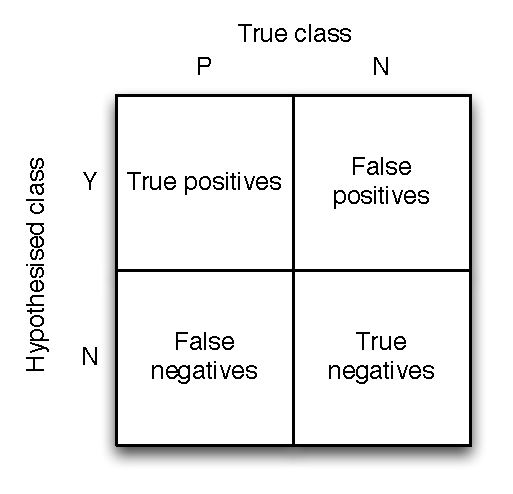
\includegraphics[height=8cm]{figures/confusion}
\end{center}
\caption{Confusion matrix for binary classification \cite{Fawcett2006}. }
\label{figconfusion}
\end{figure}

We adopt the notation from the ROC paper by Tom Fawcett and use ${Y,N}$ for output from the classifier. For true classification we use ${p,n}$ for positive and negative respectively. In case of a true positive $p$ is classified correctly as $Y$. A false positive is a $p$ classified as a $N$. A false negative is $p$ classified as $N$ and true negative is $n$ classified as $N$. ROC space in fig. \ref{figrocspace} is made by plotting the $tp_{rate}$ vs. the $fp_{rate}$. The line from $(0,0)$ to $(1,1)$ represents classification by chance. Classifiers below this line do worse than luck itself. A discrete classifier outputs either $Y$ or $N$ or in our case image is found in the database or it is not. Discrete classifiers may be compared in ROC space like in fig.\ref{figrocspace} \cite{Fawcett2006}

\begin{figure}[htb]
\begin{center}
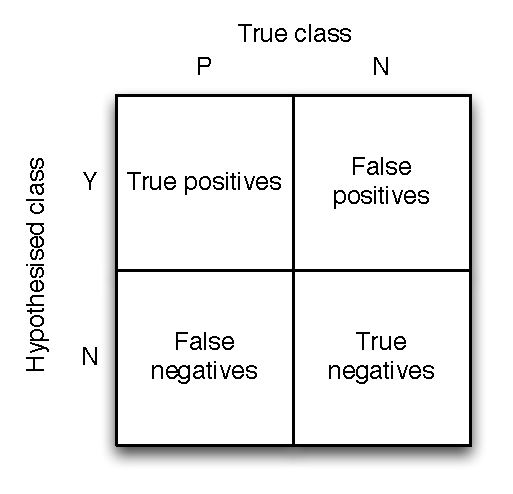
\includegraphics[height=8cm]{figures/ROC}
\end{center}
\caption{ROC space example with several discrete classifiers \cite{Fawcett2006}. }
\label{figrocspace}
\end{figure}


\begin{equation}
fp_{rate} = \frac{FP}{N}
\end{equation}
\begin{equation}
tp_{rate} = \frac{TP}{P}
\end{equation}
\begin{equation}
precision = \frac{TP}{TP + FP}
\end{equation}

\begin{equation}
recall = \frac{TP}{P}
\end{equation}

\begin{equation}
accuracy = \frac{TP + TN}{P + N}
\end{equation}

\subsubsection{Precision-Recall Curves}
ROC curves can give an overly optimistic view on an algorithms performance.

\subsection{Perceptual hashing} \label{perceptualhash}
A perceptual hash $H(I)$ of image $I$ is a bit sequence of length $L$ constructed from the image pixels such that similar images have similar hash values and different images have vastly differing hash values. According to \cite{Zauner2010}, perceptual hashing has vast modes of usage from content identification to content-based media retrieval.

In this paper we will only consider the use of a simple block mean based hash and a version of DCT based hash on content based media retrieval, more specifically the retrieval of content annotations.

More precisely perceptual hash $h$

\begin{equation}\label{hashfunction}
h = H(I)
\end{equation}

is the result of the hash function $H$ taking the image $I$ as input. $H$ has the properties in table \ref{hashcriteria}.

\def\arraystretch{1.5}
\begin{table}[htb]
\caption{Perceptual hash requirements. \cite{Zauner2010}}
\label{hashcriteria}
\begin{center}
\begin{tabular}{lp{0.5\linewidth}}
  \hline \hline
  Compression & $H$ maps from arbitrary size $I$ to fixed number of bits $m$\\
  \hline
  Fast computation & $H(I)$ fast to compute \\
  \hline
  Ease of implementation & $H(I)$ is easy to implement\\
  \hline
  Ease of understanding & $H(I)$ is easy to understand\\
  \hline
\end{tabular}
\end{center}\end{table}


In addition, according to \cite{mihccak2001new} $H(I)$ where $P$ is probability and $L$ is the length of the hash, the hash function $H$ eq. \ref{hashfunction} should
\begin{enumerate}
\item Distribute hashes equally:\\
  \begin{equation}\label{phashdistribute}
  P[H(X)=\alpha]\approx\frac{1}{2^L},\quad\forall\alpha\in \{0/1\}^L
  \end{equation}
\item Visually different images X and Y are pairwise independent: $\forall\alpha,\beta\in\{0/1\}^L$\\
  \begin{equation}\label{phashindependent}
    P[H(X)=\alpha|H(Y)=\beta]\approx P[H(X)=\alpha]
  \end{equation}
\item Approximately equal for visually similar images X, $\hat{X}$\\
  \begin{equation}\label{phashsame}
    P[H(X) = H(\hat{X})] \approx 1
  \end{equation}

\item Be different for visually different images X, Y\\
  \begin{equation}\label{phashdif}
    P[H(X)=H(Y)]\approx 0
  \end{equation}
\end{enumerate}

\subsubsection{Hamming distance}
According to \cite{Hamming1950} given alphabet $A$ the hamming distance $\Delta$ between strings $x \in A$ and $y \in A$ is

\begin{equation}\label{hammingeq}
\Delta(x,y):=\sum_{x_i\neq y_i}1\quad,\quad i=1,\ldots,n
\end{equation}

In other words, it is the number of characters two strings differ. In binary strings it is the number of bits by which two binary numbers differ. Table \ref{hammingexamples} provides some examples. The hamming distance can be used to for content based image retrieval by perceptual hashing by comparing the incoming image hash and the hashes in the database by eq. \ref{hammingeq}. If the hamming distance is within some threshold, the image can be said to be in the database.

\begin{table}[htb]
\caption{Hamming distance for strings.}
\label{hammingexamples}
\begin{center}
  \begin{tabular}{ccr}
&&$\Delta(x,y)$\\
    \hline \hline
    101 & 111 & 1\\
    \hline
    123 & 321 & 2\\
    \hline
    foo & bar & 3\\
    \hline
\end{tabular}
\end{center}\end{table}



\subsubsection{Block mean based simple hash}
According to \cite[p. 20]{Hadmi2012} the simple hash belongs in the statistic-based hashing schemes and is a simplified version of the block mean value based hash in \cite{Yang2006}.

The simple hash (eq. \ref{simplehasheq}) scales the image image to $8px * 8px$ grayscale. Then thresholding takes place where the average value of the most significant byte is found and hash bits are set to one if the image pixel MSB is greater than the average or to zero if it is less than or equal to.

More specifically the resulting hash has two parts. The most significant $64$ bits represent the image pixels and the least significatn $64bits$ represent the horizontal flip of the $8px * 8px$ grayscale image.

\begin{equation} \label{simplehasheq}
  \begin{split}
  b_{i} = 1 | I_{msB}(u,v) > px_{avg}\\
  b_{i} = 0 | I_{msB}(u,v) \leq px_{avg}
  \end{split}
\end{equation}

where $b_{i}$ denotes $ith$ hash bit where $0 \leq i < 64$ and $I_{msB}(u,v)$ is the most significant byte of pixel of $I$ at $(u,v)$ where $0 \leq u,v < 8$.

The second part (eq. \ref{simplehasheqmirror})of the hash is calculated on the mirror image of $I$ where $I_{msB}$ denotes the most significant byte of the image RGB pixel value.

\begin{equation} \label{simplehasheqmirror}
  \begin{split}
  b_{i} = 1 | I_{msB}(8-j,v) > px_{avg}\\
  b_{i} = 0 | I_{msB}(8-j,v) \leq px_{avg}
  \end{split}
\end{equation}

A simple hash is simple and fast to calculate so it meets all the criteria in table \ref{hashcriteria}. The calculation steps are in table \ref{simplesteps}. A single simple hash takes on average 70ms on Matlab 2015a on a Mid 2014 13 inch Macbook Pro.

\def\arraystretch{1.5}
\begin{table}[htb]
\caption{Simple calculation hash steps.}
\label{simplesteps}
\begin{center}
\begin{tabular}{lp{0.5\linewidth}}
  Calculation step\\
  \hline \hline
  Scale image to 8 by 8 px grayscale\\
  \hline
  64 adds\\
  \hline
  64 logical ands\\
  \hline
  one multiplication\\
  \hline
  one division\\
  \hline
  128 logical ands\\
  \hline
  128 logical ors\\
  \hline
  128 bitshifts\\
  \hline
\end{tabular}
\end{center}\end{table}

As shown in table \ref{simplesteps}, the simple hash is very simple to calculate. It is also fast as mentioned earlier. Out of the methods presented in this paper it is the fastest to understand and the fastest to implement. Yet, it should perform well for isotropically scaled images and the thresholding ensures that any uniform change to pixel data where the relationships between the pixels stay the same \cite{Zauner2010}. Any nonuniform changes to pixel values especially relating to moving pixel positions relative to the original image will perform poorly.

Content based image retrieval is done by calculating the hash of an incoming image and comparing it to the image hashes for that user. Typically the number of hashes in the set doesn not exceed 100. A hamming distance tolerance is used so the incoming image hash and a hash in the database may differ by $n$ bits where $n$ is the hamming distance.


\subsubsection{DCT based hash}
According to \cite{Gonzalez2002}, many ''transform coding systems are based on the DCT, which provides a good compromize between information packing ability and computational complexity'', properties which are in accordance with requirements for perceptual hashes in table \ref{hashcriteria}. A dct based hash is formed using a grayscale scaled version of the image, a dct transform of the scaled image and thresholding to produce a $L=64$ bit hash. Unlike the simple hash, DCT hash operates in the frequency domain. Especially the low frequency DCT image components are difficult to change without visually altering the image \cite{Fridrich1999}.

To create the hash, the image is reduced to $32$ by $32$ px grayscale. From the result, the most significant byte of the pixel (reduced image) is used. A $N =32$ DCT eq. \ref{dcteq} is applied to the reduced image and the coefficients are set according to equation \ref{dctcoefeq}.


Using only $N = 8$ (topleft corner) of the $N=32$ DCT, the average of the result is calculated and origin result value is discarded as it would throw off the average. The use of average as a threshold is unlike \cite{Coskun2004} where the median is used. The bits of the hash are set to 1 or 0 if the DCT-value is above or below average respectively according to eq. \ref{simplehasheq}.

\begin{equation}\label{dcteq}
T(u,v)= \sum_{u=0}^{N-1} \sum_{v=0}^{N-1}\alpha(u)\alpha(v)cos\left[\frac{(2x-1)u\pi}{2N}\right]cos\left[\frac{(2y + 1)v\pi}{2N}\right]
\end{equation}

\begin{equation}\label{dctcoefeq}
  \alpha(u) = \alpha(v)= \begin{cases}
    \sqrt{\frac{1}{N}} \quad \textrm{for} \quad u=0\\
    \sqrt{\frac{2}{N}} \quad \textrm{for} \quad u=1,2,\ldots,N-1
    \end{cases}
\end{equation}

The image is scaled down to 32 by 32 px grayscale and the most significant byte of the pixel is extracted. The two dimentional $N=32$ type-II DCT (eq. \ref{dcteq}) is calculated. Only the top left 8 by 8 corner of the DCT result is used. Most of the image information resides in the low frequency components (top left corner). From these 64 values the average is calculated and the origin value is dropped from the average. In figure \ref{dctkernels} we see the origin being very large compared to the rest of the DCT basis values. This throws off the average and thresholding. The 8 by 8 values are thresholded by eq. \ref{simplehasheq} into a 64 bit hash. These steps are outlined in table \ref{dctsteps}.

\begin{figure}[htb]
\begin{center}
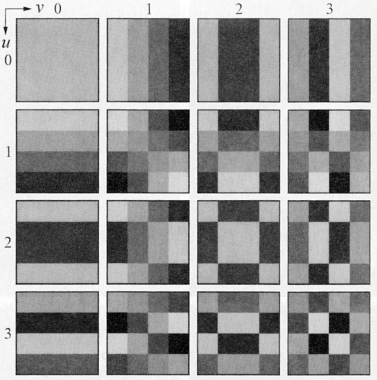
\includegraphics[height=8cm]{figures/dct}
\end{center}
\caption{Discrete-cosine basis functions for $N = 4$. The lighter the color, the larger the value. \cite[p. 473]{Gonzalez2002}}
\label{dctkernels}
\end{figure}

\def\arraystretch{1.5}
\begin{table}[htb]
\caption{DCT hash calculation steps give a good idea into its simplicity. Compare to table \ref{simplesteps} for simple hash complexity.}
\label{dctsteps}
\begin{center}
\begin{tabular}{lp{0.5\linewidth}}
  Calculation step\\
  \hline\hline
  Scale image to 32 by 32 px grayscale\\
  \hline
  $32^2\quad*\quad \&$ \\
  \hline
  $32^4 \quad*\quad \cos, 3+, 10*, 2/$ \\
  \hline
  $32^2\quad*\quad 2*, /$\\
  \hline
  $64 \quad*\quad +$\\
  \hline
  $1 \quad*\quad -$\\
  \hline
  $1 \quad*\quad /, *, -$\\
  \hline
  $64 \quad*\quad |, <<$\\
  \hline
\end{tabular}
\end{center}\end{table}

This version of DCT-Hash takes 194ms on a 13'' mid 2014 Macbook Pro and Matlab 2015b.

\subsection{Local features}
To improve upon duplicate detection by perceptual hashing, we raise the abstraction level from image pixels to an object or scene in the image itself. With hashing, the image identifier is created from the image pixels to form a binary string of fixed length. Local features however identify an object in the image by a large amount of scale-, illumination-, noise- and affine distortion invariant features.

Keypoint detectors have been widely developed in the last decade. The steps for image classification with these methods are the same.

\begin{enumerate}
\item Find keypoints of interest in image
\item Encode keypoints in a visual descriptor
\item Match incoming descriptor to all known descriptors
\end{enumerate}

Local features have been in use since Moravec invented the corner detector in the early 1980's. The Moravec corner detector was improved by Harris and Stephens by using a Gaussian window function instead of the binary window used by Moravec. The Harris detector was not scale invariant, which lead David Lowe to come up with the scale invariant feature transform (SIFT). SIFT has inspired many similar methods including Sped Up Robust Features (SURF), and BRISK and ORB which are not covered here. We will cover KAZE, and AKAZE features more recent techniques using local features.

Scale-invariant features identify the image by a large set of local descriptors that are chosen so that they are invariant to image scale, rotation, viewpoint change, distortion and difference in lighting. The descriptors also remain stable under some degree of affine distortion. \cite{Lowe2004}

We are expecting to improve over perceptual hashes which withstand scaling extremely well. However they are weak under image transformations that alter the relationships betwen pixel values such as rotaition and adding and removing from the image. Feature matching in a large feature database is enabled by highly distinctive features.

\subsubsection{Scale Invariant Feature Transform}
Scale Invariant Feature Transform or SIFT ''transforms image data into scale-invariant coordinates relative to local features \cite{Lowe2004}''. SIFT descriptors are suitable for matching images of the same object or scene. They are robust to image scaling, rotation and somewhat robust to change in viewpoint, scene lighting and affine distortion. A large number of descriptors can be computed on ''off the shelf''-hardware in near realtime. \cite{Lowe2004}

A SIFT-descriptor has a location $t_x, t_y$ a scale $s$ and rotation $\theta$. A SIFT-descriptor is the vector $(s, \theta, t_x, t_y)$. Examples of SIFT features can be seen in fig. \ref{siftfeatures}.

SIFT descriptors are extracted by

\begin{enumerate}
\item Scale space extrema detection identifies scales and locations that can be repeatedly extracted under changing conditions.
\item Keypoint localization
\item Orientation assignment
\item Keypoint descriptor
\end{enumerate}
\cite{Lowe2004}

\begin{figure}[htb]
\begin{center}
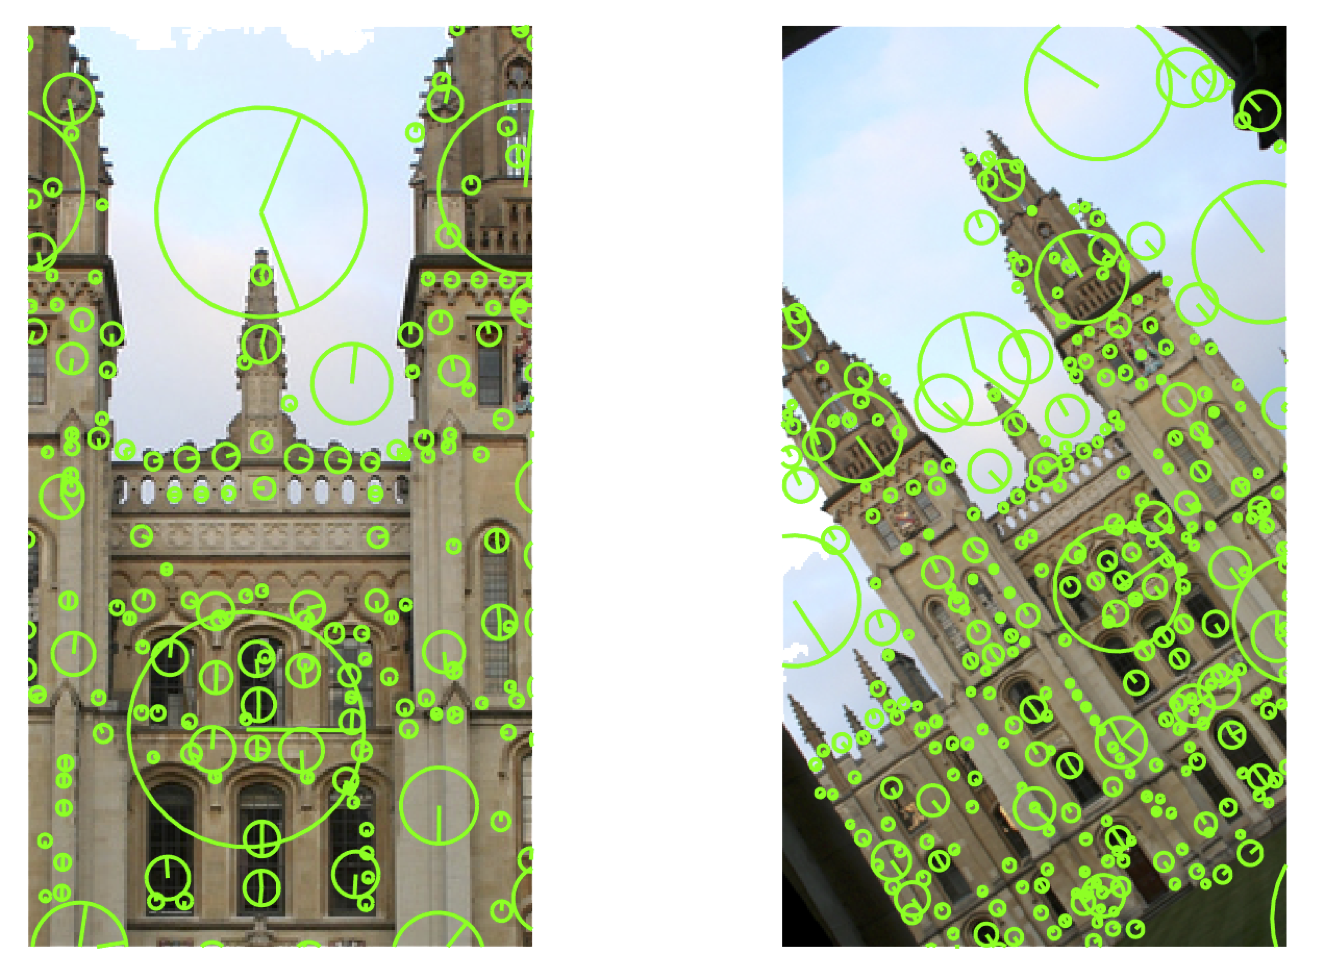
\includegraphics[height=8cm]{figures/siftDescriptor}
\end{center}
\caption{Visualized SIFT-descriptors.}
\label{siftfeatures}
\end{figure}

To find scale space extrema $D$, a difference-of-Gaussian function is convolved with the image $I$.
\begin{equation}\label{keypoints}
  D(x,y,\sigma) = (G(x,y,k\sigma) - G(x, y, \sigma))*I(x,y)
\end{equation}\cite{Lowe2004}

$G(x,y,k\sigma) - G(x, y, \sigma)$ may be approximated by a normalized Laplacian so

\begin{equation}\label{approximatedog}
G(x,y,k\sigma) - G(x, y, \sigma) \approx (k - 1)\sigma^{2}\nabla^{2}G
\end{equation}\cite{Lowe2004}

where the right hand side is a scale-normalized Laplacian of Gaussian.

$D$ are keypoint candidates. The robust keypoints are weeded out by fitting them to the surrounding data. \cite{Lowe2004} Adding the offset

\begin{equation}\label{keypointoffset}
\hat{\boldsymbol{x}} = - \frac{\partial^2D^-1}{\partial \boldsymbol{x}^2}\frac{\partial D}{\partial \boldsymbol{x}}
\end{equation}\cite{Lowe2004}

\subsubsection{Speeded Up Robust Features}
Speeded Up Robust Features (SURF) was for fast computation of the the detector and descriptor than state-of-the-art methods of the time. SURF introduces the 'Fast-Hessian' detector that relies on box filter approximations of Gaussian filters and integral images to reduce the computation time. \cite{Bay2006} An integral image $ii(x,y)$ (eq. \ref{integralimage})

\begin{equation}
  \label{integralimage}
ii(x,y) = \sum\limits_{x'\le,y'\le y} i(x', y')
\end{equation}

at point $x, y$ sums up the pixels above and below where $i(x,y)$ is the source image. \cite{Viola2001}

\begin{equation}
  \label{integralimagerowsum}
s(x,y) = s(x, y - 1) + i(x,y)
\end{equation}

\begin{equation}
  \label{integralimagepartial}
  ii(x,y) = ii(x-1,y) + s(x,y)
\end{equation}

The integral image is very quick to calculate using the cumulative row sum $s(x,y)$ (eq. \ref{integralimagerowsum}) and recurrence (best viewed in figure \ref{integralimagefig}) within integral images (eq. \ref{integralimagepartial}) where $s(x, -1) = 0$ and $ii(-1,y)=0$. A rectangular sum follows from four array references in figure \ref{integralimagefig}.

\begin{figure}[htb]
\begin{center}
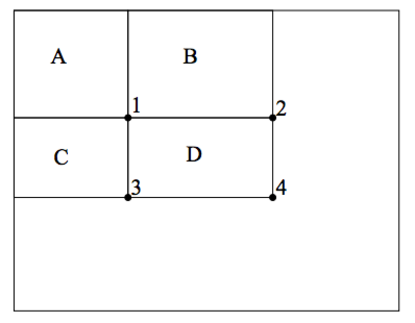
\includegraphics[height=8cm]{figures/integralimage}
\end{center}
\caption{Rectangular sums from integral images. Point 1 is the sum of pixels in A. Point 4 is $A + B + C + D$.\cite{Viola2001}}
\label{integralimagefig}
\end{figure}

The calculation of the descriptor also uses integral images for speed. The descriptor is a distribution of Haar-wavelet reponses within the interest point neighbourhood. \cite{Bay2006}

The orientation of the descriptor is determined by Haar-wavelet responses in $x$ and $y$ directions in the scale $s$ that the keypoint was detected with $6s$ radius at sampling step size also $s$. Wavelet size is $4s$. Responses are weighted with a Gaussian $(\sigma = 2.5s)$ at the interest point. The dominant direction is estimated by summing up the responses over a sliding window angle of $\frac{\pi}{3}$. The horizontal and vertical results are summed to form a new vector and the longest vector angle is the orientation of the interest point. The SURF descriptor is a square region centered on the interest point. \cite{Bay2006}

The size of the region is $20s$ and is split into $4 \times 4$ sub-regions. Let $d_x$ and $d_y$ be Haar wavelet responses in along horizontal and vertical region edges respectively. For robustness, the responses are weighted with a Gaussian $(\sigma = 3.3)$ and $d_x, d_y$ are summed independently to form the first part of the sub-region descriptor in eq. \ref{surfdescriptor}. \cite{Bay2006}

\begin{equation}
  \label{surfdescriptor}
v = (\sum d_x, \sum d_y, \sum \abs{d_x}, \sum \abs{d_y})
  \end{equation}

The second part of the descriptor, $\sum \abs{d_x}, \sum \abs{d_y}$ accounts for sizes of polarity changes. As each region is divided into $4 \times 4$ subregions, each region generates a 64 length descriptor. Normalization to a unit vector provides scale invariance while the wavelet responses are invariant to luminance changes. \cite{Bay2006}

Matching requires fast indexing and additionally storing the sign of the Laplacian for the interest point speeds up searches. The 'Fast-Hessian' detector in the SURF paper was found to be three times faster than the DoG detector by Lowe used in SIFT. SURF improved over SIFT in recall by $4.5\%$. \cite{Bay2006}

\subsubsection{KAZE Features}
KAZE improves SIFT with nonlinear diffusion filtering in place of the difference of Gaussians scale space for detecting relevant features. Nonlinear diffusion filtering maintains or enhances edges \cite{Weickert1998}. There is no downsampling of the scale space like in SIFT. The computation time is simlar to SIFT but slower than SURF. Gaussian blurring in Gaussian scale space blurs detail and noise alike. Nonlinear diffusion filtering by Additive Operator Scaling however builds the scale space in a way which that reduces noise and leaves object boundries unblurred leading to improved localization accuracy and distinctiveness. Computation time is comparable to SIFT and slower than SURF. The name KAZE, Japanese for wind, is a tribute to Iijima, inventor of scale space analysis. For KAZE features one must

\begin{enumerate}
\item build nonlinear scale space using Additive Operator Splitting
\item detect interesting 2D features via maxima of a scale-normalized determinant of Hessian response through the nonlinear scale space
\item compute M-SURF descriptor orientation and scale from first order image derivatives.
\end{enumerate}

The nonlinear diffusion equation (eq. \ref{nonlineareq}) where $L$ is the luminance, $c$ is the conductivity function and by choosing this conductivity function in a good way the diffusion will adapt to the image structure $x, y$ and is dependent also on time $t$, which is the scale parameter. When $t$ is large, the filtered image is simpler. \cite{Alcantarilla2013}

\begin{equation}
  \label{nonlineareq}
  \frac{\partial L}{\partial t} = \nabla \cdot c(x,y,t)\cdot\nabla L
\end{equation}
\cite{Alcantarilla2012}

The conductivity function eq. \ref{conductivityfunceq} has the image gradient magnitude controlling the diffusion

\begin{equation}
  \label{conductivityfunceq}
c(x,y,t)=g(\abs{\nabla L_\sigma(x,y,t)})
\end{equation}

Perona and Malik covered several conductivity functions in \cite{Perona1990} and we will focus on $g_2$ (eq. \ref{gtwoeq}) which creates the best overall classifiers according to data in \cite{Alcantarilla2012}. $\lambda$ is a contrast factor and controls the level of diffusion where $\nabla L_{\sigma}$ is the gradient of a Gaussian smoothed source image.

\begin{equation}
  \label{gtwoeq}
g_2 = \frac{1}{1 + \frac{\abs{\nabla L_\sigma}^{2}}{\lambda^{2}}}
\end{equation}

$\nabla L_{\sigma}$ can be regarded as the edge detector where if $\abs{\nabla L_{\sigma}} > \lambda$ an edge has been encountered. If $\abs{\nabla L_{\sigma}} < \lambda$ we are dealing with a region and diffusivity (filtering) is increased. \cite{Weickert1998}


\subsubsection{Accelerated KAZE Features}
The main drawback of KAZE features is building the nonlinear scale space by nonlinear diffusion filtering.  The KAZE method of choice is Additive Operator Scaling (AOS). AOS requires solving a large system of linear equations, which is computationally intensive. A-KAZE features solves this problem by replacing AOS in KAZE with Fast Explicit Diffusion (FED) reducing computation time of the nonlinear scale space. In addition, AKAZE uses a Modified-Local Difference Binary (M-LDB) descriptor over M-SURF descriptor used in KAZE.

Fast Explicit Diffusion (FED) is able to build the nonlinear scale space faster than AOS. AKAZE improves in speed over KAZE-, SURF-, and SIFT features. ''Fast explicit diffusion (FED) schemes perform cycles of explicit schemes with varying time step sizes that may violate the stability restriction in up to 50 percent of all cases.''\cite{Grewenig2010}

FED is equivalent to box filtering and can approximate Gaussian kernels with good quality and is easy and fast to implement. Factorization of the box filter

\begin{equation}
  \label{boxfilterfactor}
\tau_j = \frac{\tau_max}{2cos^2\left( \pi \frac{2j+1}{4n+2}\right)}
\end{equation}

where $n$ is the number of explicit diffusion steps, $\tau_{max}$ is the maximal step size that does not violate the stability condition of the explicit scheme.

The FED cycle stopping time $\theta_n$

\begin{equation}
\theta_n = \sum_{j=0}^{n-1}\tau_j=\tau_{max}\frac{n^2+n}{3}
\end{equation}

Equation \ref{nonlineareq} can be discretized as

\begin{equation}
  \label{discretenonlineareq}
\frac{L^{i+1}-L^i}{\tau}=A(L^i)L^i
\end{equation}

where

\begin{equation}
  \label{fednextevolution}
  L^{i+1}=(I + \tau A(L^i))L^i
\end{equation}

$A(L_i)$ is the image conductivity matrix and $\tau$ is the constant step size on condition $\tau < \tau_{max}$ to meet stability conditions.

FED cycles while building the scale space are run from short to long. A scale space consists of $O$ octaves (index $o$) and $S$ (index $s$) sub-levels. Scale $\sigma$ is

\begin{equation}
  \label{scalespace}
  \sigma_i(o,s) = 2^{o+s/S},o \in[0\ldots O-1], s \in [0\ldots S-1], i \in [0 \ldots M]
  \end{equation}

where $M$ is the total number of filtered images.

\begin{equation}
  \label{scaletotime}
t_i = \frac{1}{2}\sigma^2_i,\{i=0\ldots M\}
\end{equation}

To reduce noise the source image may be processed with a Gaussian of $\sigma_0$. The contrast factor $\lambda$ is the 70th percentile of the input image gradient histogram.

The pyramidal FED scheme has an outer loop and an inner loop. The inner loop performs the filterign according to step sizes set by the outer loop. The outerloop also takes care of downsampling with mask $(\frac{1}{4}, \frac{1}{2}, \frac{1}{4})$. The downsampled image is the input to the next octave. For 2D images the maximum step size is $\tau_{max}$ when the image derivative grid size is 1px. The contrast parameter $\lambda$ also needs to be modified for each octave as the downsampling mask reduces contrast by 25\%.

A Hessian (eq. \ref{akazehessian}) is calculated for each $L^i$

\begin{equation}
  \label{akazehessian}
L^i_{Hessian} = \sigma^2_{i,norm}(L^i_{xx}L^i_{yy}-L^i_{xy}L^i_{xy})
\end{equation}

to obtain features. Scharr filters with step size $\sigma_{i,norm}$ are used to compute the second order derivatives.

In order to be accepted as a feature location, a maxima has to

\begin{enumerate}
\item in a $3 \times 3$ window where it has to be a maxima
\item it has to be greater than a threshold
\item it is maxima at level $i+1$ and $i-1$ in a $\sigma_i\times\sigma_i$ window
\end{enumerate}

After detection the precise interest point location is found by fitting a 2D quadratic function to the determinant of the Hessian response in the neighbourhood of $3 \times 3$ px and finding the maximum.

A-KAZE uses a Modified Local Difference Binary descriptor. The LDB descriptor is modified to speed up calculations relating to rotation invariance.

LDB stores intencity, means of the horizontal and vertical derivatives. LDB uses grids of finer steps dividing the descriptor into subgrids. M-LDB rotates these LDB grids to the interest point orientation. Due to this rotation, integral images may not be used to calculate averages of pixels inside the subgrids, the subgrids are subsampled in steps which are a function of the scale $\sigma$ M-LDB re-uses the derivatives from the detection step in the descriptor.

\lstinputlisting{fed.m}

\subsection{Large Scale Image Retrieval}

When all the descriptors in the database do not fit into system RAM, the efficiency of the retrieval system collapses due to disk access \cite{Philbin2007}.

In order to match amongst a large number of images, the descriptors are quantized into visual words to speed up the search. In order to further optimize search, the descriptor format is optimized for memory and computation speed. \cite{Jegou2010}

\subsubsection{Nearest Neighbor Search}
Matching a new image descriptor to a set of known image descriptors can be as simple as a Euclidean nearest neighbor search (eq. \ref{nneq}) which Donald Knuth also named as the \emph{post-office problem} in vol. 3 of The Art of Computer Programming (1973). It answers the question ''To which post office does this address belong to?'' which is analogous to ''which known image descriptor is closest to this new image descriptor?''.

Matching in a set of millions of images is not feasible in user facing applications as the time complexity is $\mathcal{O}(nd)$ where $n$ is the number of image descriptors in the set and $d$ is the dimentionality of each image descriptor.


\begin{equation}
\label{nneq}
NN(x) = arg \min_{y\in Y}\norm{x-y}^2
\end{equation}

\begin{figure}[htb]
\begin{center}
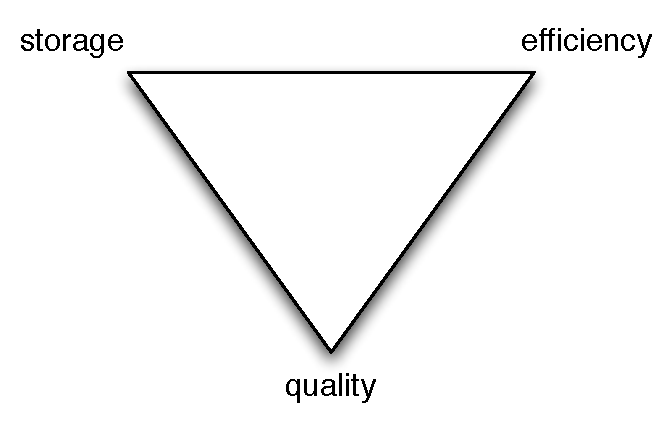
\includegraphics[height=4cm]{figures/nntradeoffs}
\end{center}
\caption{Tradeoffs for improving nearest neighbor search}
\label{nntradeoffs}
\end{figure}

To improve scalability, one can relax the conditions on nearest neighbor. The tradeoffs involved (fig. \ref{nntradeoffs}) are memory footprint, as the descriptors the faster the memory the descriptors are stored in, the more computationally feasible matching becomes at large scale. Increasing the quality of the matches will require sacrifices in speed and the memory footprint. Aprroximate nearest neighbor mehtods are able to solve the ''curse of dimensionality'' in many cases.

Approximate nearest neighbor is defined as in a normed space $l_p^d$ preprocess set of points $P$ to efficiently return a point $p\in P$ for any given query point $q$, such that $d(q,p) \lq (1 + \epsilon)d(q,P)$. $d(q, P)$ is the distance between the closest point in $P$ to $q$. \cite{Gionis1999}

\subsubsection{Locality Sensitive Hashing}
The original SIFT descriptor has 128 dimensions \cite{Lowe1999}.  The SURF descriptor has 64 dimensions. Since the Nearest Neighbor search (eq. \ref{nneq}) time complexity is dependent on the descriptor dimension $d$, a search in 5 million images scales linearly (poorly). Locality Sensitive Hashing was developed to solve this ''curse of dimensionality'', where $d > 3$ for NN search \cite{Gionis1999}. LSH scales well for $d > 50$ \cite{Gionis1999}. We will only cover the main idea behind the LSH family of methods. A review of the state of the art in 2008 can be found in \cite{Andoni2008}. Finding optimal hash functions for LSH applications has attracted much more recently so we examine \emph{Optimal LSH for Angular Distance} \cite{Andoni2015} by Andoni et al. from 2015.

For hash function $g$ to be Locality-Sensitive, the probability of collision is higher for points that are nearby than for those that are fare away \cite{Andoni2015}.

Hash function quality can be described by $p_1$, the collision probability for points close to each other and $p_2$ the collision probability for distant points \cite{Andoni2015}. Naturally difference between $p_1$ and $p_2$ characterizes hash function reactivity to changes in distance better described by $\rho$ (eq. \ref{lshsensitivity}).

\begin{equation}
  \label{lshsensitivity}
  \rho = \frac{log\frac{1}{p_1}}{log\frac{1}{p_2}}
  \end{equation}

The goal of LSH is to hash data points in a way so the probability of collision is high for points close to one another compared to points that are far apart. By allowing for small error (eq. \ref{lsherroreq}) in the results and adding to storage requirements, the query time is significantly improved, giving up quality for speed as seen in fig. \ref{nntradeoffs}. \cite{Gionis1999} The solution presented in \cite{Gionis1999} reduces ANN time complexity to $\mathcal{O}(dn^{\frac{1}{1+\epsilon}})$.

LSH has $m$ hash functions, hash tables and keys per vector. Each point in the set $P$ has $m$ hash keys as an index. At query time $m$ keys are computed on the query vector and all the vectors associated with the new keys are retrieved forming a shorter list where it's feasible to use exact distance for matching.

\lstinputlisting{lshinit.m}

\lstinputlisting{lshquery.m}

For the Approximate 1-NNS problem the effective error $E$ is

\begin{equation}
  \label{lsherroreq}
E = \frac{1}{\abs{Q}}\sum_{q\in Q}\frac{d_{LSH}}{d^*}
  \end{equation}

where $d^*$ is the distance from $q$ to the nearest point over all successful queries.


\subsubsection{min-Hash}
min-Hash was used in \cite{Broder1997} to search for similar text documents amongst 30 million documents. In \cite{Chum2008} the same idea is harnessed to find duplicate images for sample data sets. \cite{Chum2010} Uses min-Hash techniques to find duplicates in $10^4, 10^5$ and $5 \times 10^6$ images. It finds similar images with a probability near to one, near similar images with small probability and unrelated images with 0 probability \cite{Chum2010}.

Essentially it is LSH for sets \cite{Chum2010}. Like in the case of perceptual hashes (section \ref{perceptualhash}), two images are considered alike if the result of some similarity function $sim_s$ is higher than some threshold \cite{Chum2008}. In \cite{Chum2008}, it quantizes and compresses SIFT descriptors. It is included in the retrieval section, as the major contributions lie in the retrieval step for finding near duplicate objects. It solves issues of storage and efficiency in a proven way for moderately large datasets.

The corner stone is min-Hash ability to estimate document or image similarity based on a set of data significantly compressed from the original data set.

Considering the 128 dimentional SIFT descriptor and 10 million images, if one uses 400 independent hash functions $f_j:\mathcal{V} \rightarrow R$, $f_j, i = 1 \ldots 400$, the similarities are evaluated on a dataset with 128 columns but only 400 rows.

min-Hash (eq. \ref{minhash}) is the smalles element of set $\mathcal{A_i}$ under ordering by $f_j$

\begin{equation}\label{minhash}
m(\mathcal{A}_i,f_j)= arg \min_{X \in \mathcal{A}_i}f_j(X). \quad \cite{Chum2008}
\end{equation}

It estimates object (text or image) similarity based on (eq. \ref{minhash}) the probability (eq. \ref{minhashsim}) that sets $\mathcal{A}_1$ and $\mathcal{A}_2$ have equal min-Hashes is the same as their similarity (eq. \ref{similarityminhash}) \cite{Chum2008}. The used similarity function can vary. Set similarity or Jaccard is similarity demonstrated in eq. \ref{similarityminhash}

\begin{equation}\label{similarityminhash}
sim_W(\mathcal{A}_1,\mathcal{A}_2) = \frac{\abs{\mathcal{A}_1 \cap \mathcal{A}_2}}{\abs{\mathcal{A}_1 \cup \mathcal{A}_2}}
\end{equation}

 and for images drawing inspiration from the \emph{tf-idf} scheme a histogram instersection approach

\begin{equation}\label{similarityminhashimages}
sim_h(\mathcal{A}_1, \mathcal(A)_2)=\frac{\sum_W min(t^w_1,t^w_2)}{\sum_W max(t^w_1,t^w_2)}
\end{equation}

where $t_i$ is size $\abs{\mathcal{V}}$ and $t_i^w$ of the $i$-th document is the count of visual word $X_w$ in that document. $d_w \geq 0$ is the importance of $X_w$. This similarity measure performed better in efficiency and quality than Jaccard distance for the TrecVid 2006 data set. \cite{Chum2008}

\begin{equation}\label{minhashsim}
P(m(\mathcal{A}_1,f_j) = m(\mathcal{A}_2,f_j)) = \frac{\abs{\mathcal{A}_1 \cap \mathcal{A}_2}}{\abs{\mathcal{A}_1 \cup \mathcal{A}_2}} = sim_s(\mathcal{A}_1, \mathcal{A}_2)
\end{equation}

Just as a set of words was used in \cite{Broder1997}, to borrow the BoW approach from section \ref{BOW}, an image can be represented as a set of visual words and the min-Hash can be applied to NDID. More specifically, with vocabulary $\mathcal{V}$, an image is represented by a vector of length $\abs{\mathcal{V}}$ containing the number of features falling on a given visual word \cite{Chum2008}.

To ease retrieval the min-Hashes are organized into \emph{sketches} \cite{Chum2008}, \cite{Broder1997}

\begin{equation}\label{sketch}
(m(\mathcal{A_1},f_1) \ldots m(\mathcal{A_1},f_n))
\end{equation}

which have similarity

\begin{equation}\label{sketchsim}
sim_s(\mathcal{A}_1, \mathcal{A}_2)^n \cite{Chum2008}.
\end{equation}

Sketching reduces the number of false positives retrieved by min-Hash \cite{Chum2008}. The sketch similarity is evaluated first, and only if it is above some threshold the full similarity $sim_s(\mathcal{A}_1, \mathcal{A}_2)$ is evaluated \cite{Chum2008}. The probability $P(\mathcal{A}_1 \sim^h \mathcal{A}_2)$ of sets $\mathcal{A}_1$ and $\mathcal{A}_2$ having at least $h$ identical sketches from $k$ picked

\begin{equation} \label{sketchsimilarityprob}
P(\mathcal{A}_1 \sim^h \mathcal{A}_2) = \sum_{i=h}^k \binom{k}{i} p^{in}(1-p^n)^{k-i} \quad \cite{Chum2008}.
\end{equation}
\cite{Chum2008} modifies the similarity measure with ideas borrowed from \emph{tf-idf} weighting like in \cite{Sivic2003}. This is done by including each occurrence of a visual word in the representative set for the image in question as a unique member of the set resulting in an \emph{idf} like method \cite{Chum2010}. In the TrecVid 2006 data set, and University of Kentucky database cases it distanced dissimilar documents further apart when common visual words have low \emph{idf} and are weighted down as a result leading to a lower number of sketch hits and better quality search results \cite{Chum2008}. However, \cite{Chum2008} leaves min-hash performance for very large image databases (millions of images) for further research.

Querying large sets of images is considered in \cite{Chum2010} where min-Hash is used for fast detection of duplicate images. This is done by using min-Hash for detection of random pairs of image with spatial overlap. These are named cluster seeds which are then used as queries to find similar images including the seed. In other words

\begin{enumerate}
\item store descriptors in a hash table where the probability of an image being in the same bin is the same as their similarity
\item calculate exact similarity for images falling into the same bin
\item if pair of images pass the similarity test, check spatial consistency
\item if image pair passes step 3., they become cluster seeds \cite{Chum2010}.
\end{enumerate}

Their requirements are similar to what is attempted in this paper.

\begin{enumerate}
\item scalable to tens of millions of images
\item adding new images to the dtabase is possible without recomputing the entire cluster
\item easy to parallellize
\item probability of recall is independent of cluster size \cite{Chum2010}.
\end{enumerate}

For querying the Oxford Landmark dataset, the seed generation and seed growing steps to find a match took 0.014s per image on a single 2.4GHz core for 100k images. For 5M images clustering took 0.02s per image on a 3GHz single core PC \cite{Chum2010}.

Growing the dataset size in a min-Hash database takes $\mathcal{O}(NL)$ where $N$ is the dataset size and $L$ to be the number of images in the cluster \cite{Chum2010}. The seed generation is $\mathcal{O}(N^2)$ for infinite size databases but is linear for $N \leq M$ where $M$ is the number of bins in the hashing table.

In \cite{Lee2010} a high $FP$-rate is a serious problem for large dataset. Another problem for direct image retrieval is low recall \cite{Chum2010}.

\subsubsection{Bag-of-Visual Words}\label{BOW}
Bag of words approach to describing images was developed by Sivic and Zisserman in 2003 by mimicking the approach of text searches into text documents. This is an approach not unlike the Google search engine. Their results show that there is no penalty from using search by visual words vs. n-nearest neighbor methods.\cite{Sivic2003}

To calculate image descriptors two types of viewopint covariant regions are formed. The first stage iteratively finds an elliptical region around an interest point. The result is an ellipse with a center, shape and scale. Scale comes from a local extremum of a Laplacian. The shape comes from maximizing intensity gradient isotropy over the elliptical region. This is achieved using Shape Adapted (SA) regions.\cite{Sivic2003}

The second type of region used is the Maximally Stable (MS) region. For these regions are the region area stays constant as the intensity threshold is changed.

The two types of regions complement each other in image detection. The SA regions perform well on corners and the MS regions perform well on high contrast blobs. \cite{Sivic2003}

The original BoW approach uses SIFT-descriptors introduced by Lowe. The second type of region is implemented in affine covariant regions.

BoW relies on quantizing descriptors into visual words for efficient retrieval. Descriptors are quantized by associating them with the nearest cluster of descriptors. The vector quantization is implemented by k-means clustering. \cite{Sivic2003} The original BoW implementation worked on video, but we will apply the simple image case only. In the original implementation, the Mahalanobis distance is used as the distance function in k-means clustering.

In text retrieval a document is stored in a vector of word frequencies. A weight is usually applied to the vector. Term frequency-inverse document frequency, $tf-idf$ (eq. \ref{tfidf}) is a weighting scheme common in text retrieval. In $k$ words, each document is represented by a $k$-vector $V_{d}=(t_{1},...,t_{k})^{T}$

\begin{equation}\label{tfidf}
t_{i} = \frac{n_{id}}{n_{d}}log\frac{N}{n_{i}}
\end{equation}

with $n_{id}$ is word $i$ appearing $n$ times in document $d$ and $n_{d}$ is the total number of words in document $d$. $n_{i}$ is the total number of occurrences of term $i$. $N$ is the total number of documents. The first term is word frequency and the second term is inverse document frequency. Word frequency weighs words occurring often in a document while inverse document frequency down weights words that appear often in all documents. This weighting scheme outperformed the binary and $tf$ weighting schemes\cite{Sivic2003}

\begin{equation}\label{bowrank}
  Rank = \frac{1}{NN_{rel}}\left(\sum{i=1}{N_{rel}}R_{i}-\frac{N_{rel}(N_{rel} + 1)}{2}\right)
\end{equation}

where $N_{rel}$ is the number of relevant images for particular query image, $N$ is the total number of images and $R_{i}$ is the $i$th image rank. $Rank$ is a number between 0 and 1.

Retrieval uses an inverted file where each word has a hit list for all occurrences of the word in all documents. In the visual word case, each visual word has knowledge of the image it is found in. The document vector is sparce and the retrieval is very fast.

The user specifies an area of interest in a frame and descriptors are calculated for stable regions. The descriptors are then quantized into visual words. A stop list filters out all visual words which occur frequently. Sivic and Zisserman found their case to work best dropping top 5\% and bottom 10\% of words.

Google gives additional weight to words in the search that appear close together in the retrieved document. With visual words, the retrieval is done per frame (image) only and the results are re-ranked based on spatial consistency.

A loose definition would be to require neighboring matches in query image to lie close together also in the retrieved frame.

\subsubsection{Product Quantization} \label{PQ}

\begin{equation}
  \label{quantizereq}
d(x,y)^2 \approx d(x,q(y))^2
\end{equation}

where $x$ is the query vector, $y$ is the database vector and quantizer function is $q(y)$. The error on estimated distance is bound by the quantization error, $e_d \leq e_q$.  \cite{Jegou2014}

The quantizer should be fast enough and precise. The database vector $y$ is split $y \rightarrow [y_1 \ldots y_m]$ each of which is quantized $[q(y_1)\ldots q(y_m)]$. For example, and eight dimentinal vector can be split into four subvectors each in two dimensions. In effect were using $8^4$ centroids with a quantization cost equivalent to using eight centroids. Splitting up the query vector make quantization fast. \cite{Jegou2014}

In order to query amongst

In \emph{asymmetric distance computation} (ADC) in eq. \ref{adceq}, the database vectors $y$ are quantized but the query is not. This achieves lower distance distortion over the quantized query case (fig. \ref{nosdc}) called \emph{symmetric distance computation} (SDC) not covered here. Distance $d(x,y)$ approximation $\tilde{d}(x,y)$

\begin{equation}
  \label{adceq}
  \tilde{d}(x,y)=d(x, q(y))=\sqrt{\sum_jd(u_j(x),q_j(u_j(y)))^2}
\end{equation}

$d(u_j(x),c_{j,i}) : j = 1\ldots m,i=1\ldots k^*$ are computed prior to the query. Since the square root is monotonically increasing it can be left uncalculated as the ranking of database vectors remains the same regardless of the square root\cite{Jegou2011}

\begin{figure}[htb]
\begin{center}
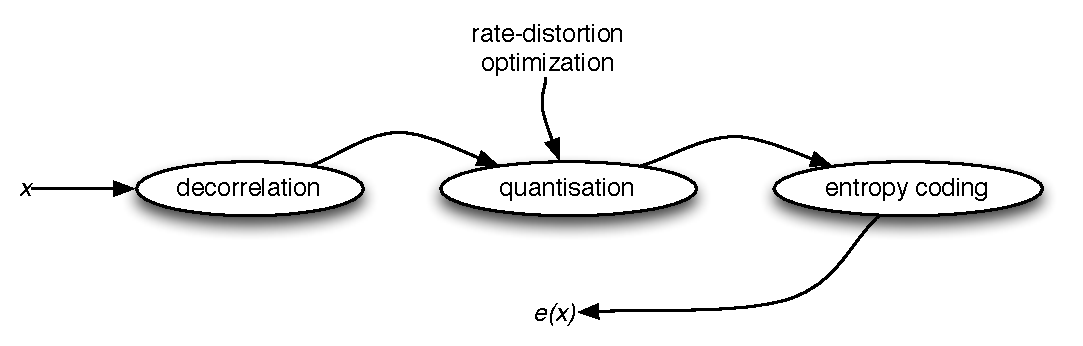
\includegraphics[height=4cm]{figures/pq}
\end{center}
\caption{Simple product quantizer \cite{Jegou2014}}
\label{pqfig}
\end{figure}

\begin{figure}[htb]
\begin{center}
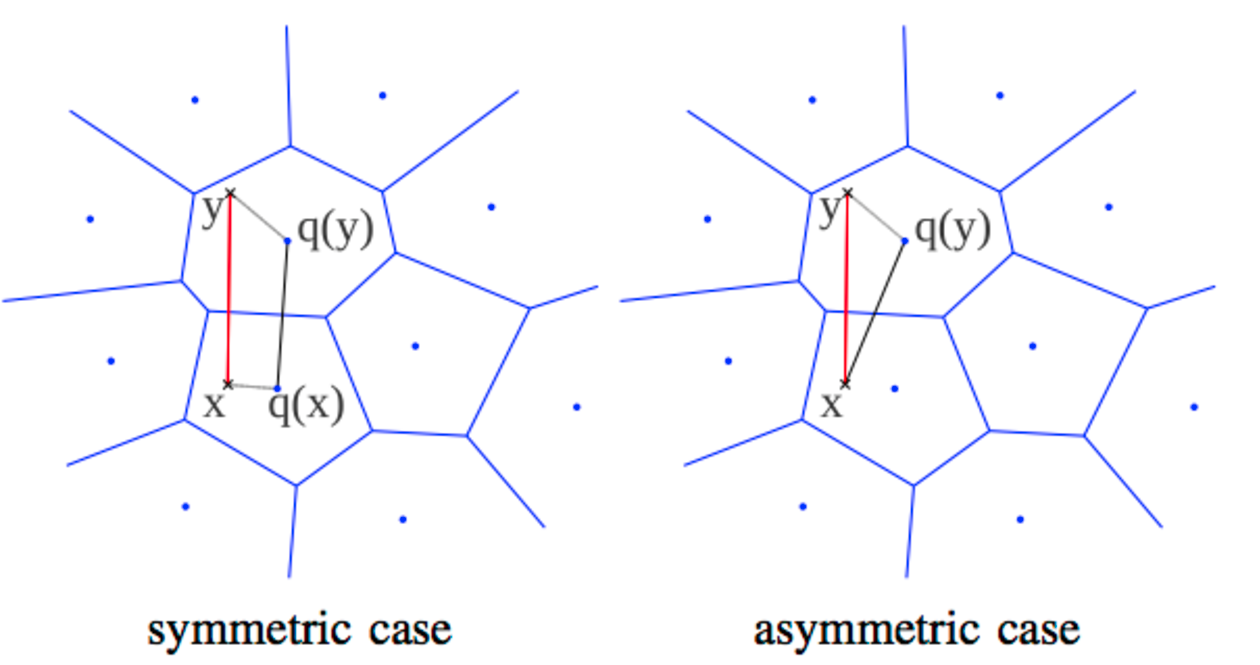
\includegraphics[height=8cm]{figures/sdcadc}
\end{center}
\caption{The increased distance distortion in the symmetric case (SDC) vs. the asymmetric case (ADC) introduced by the extra quantization $q(x)$. \cite{Jegou2008}}
\label{nosdc}
\end{figure}

ANN search with ADC is fast and reduces memory usage with some sacrifice in quality. The search is exhaustive and scales global image description well. If local descriptors are considered, exhaustive search is not feasible due to multiple queries and billions of descriptors \cite{Jegou2008}. In order to make search with local descriptors, the inverted file system from \cite{Sivic2003} is used forming an \emph{inverted file system with asymmetric distance computation} (IVFADC) (fig. \ref{ivfadcfig}).

\begin{figure}[htb]
\begin{center}
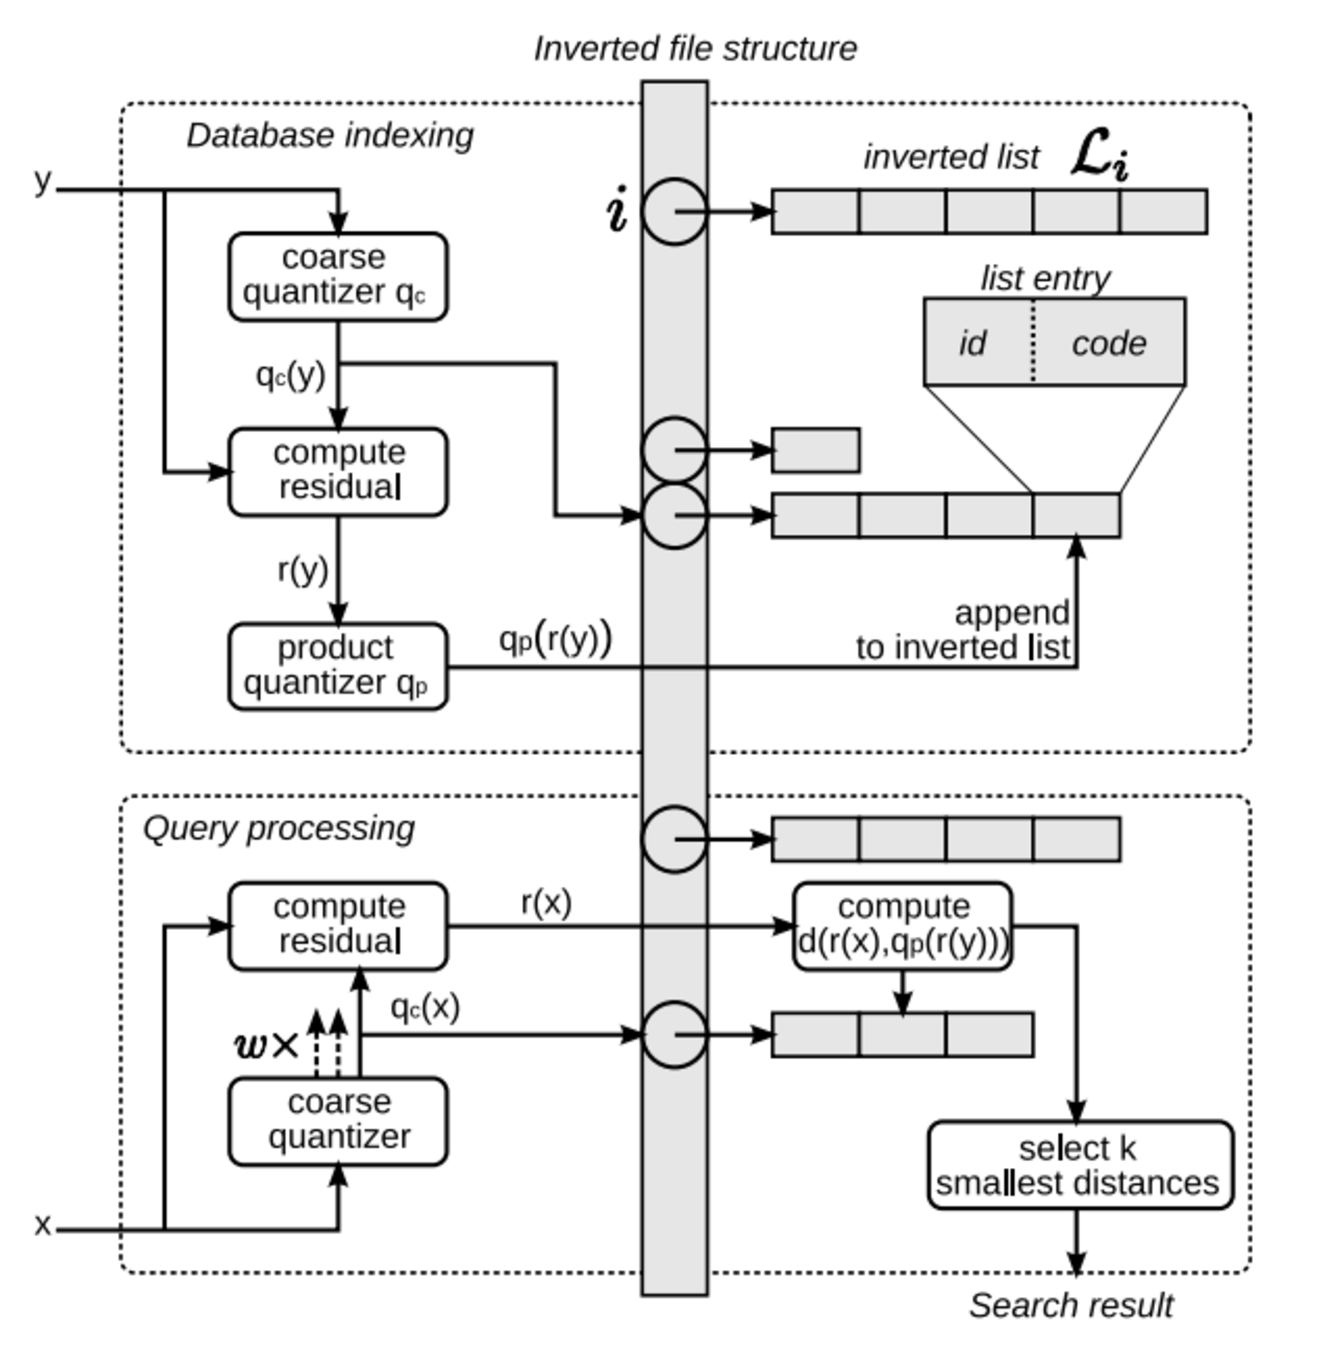
\includegraphics[height=8cm]{figures/ivfadc}
\end{center}
\caption{Block diagram of inverted file with asymmetric distance computation (IVFADC) system. \cite{Jegou2008}}
\label{ivfadcfig}
\end{figure}

The inverted file allows to rapidly access a short list of images close to the query \cite{Jegou2008}. An inverted file entry has and image index and an encoding of the difference between the query vector and the coarse centroid (table \ref{ivfadcentry}).

To set up the inverted file, the coarse quantizer $q_c$ which assigns queries to $\mathcal{L}_i$ is learned using k-means clustering. $1000 \leq k' \leq 1000000$ for SIFT descriptors \cite{Jegou2008}. A product quantizer $q_p$ like in \cite{Sivic2003} is used to encode a residual vector $r(y)$ between the coarse quantized centroid $q_c(y)$ and the vector $y$ (eq. \ref{ivfadcres}). ANN distance $\ddot{d}$ in this scenario where product subquantizers $q_{p_j}$ (eq. \ref{ivfadcestimate}). The distances between $u_j(x-q_c(y))$
and product quantizer $q_{p_j}$ centroids $c_{i,j}$ are computed in advanced and stored in lookup tables. \cite{Jegou2008}

\begin{equation}
  \label{ivfadcres}
r(y) = y - q_c(y)
\end{equation}

\begin{equation}
  \label{ivfadcestimate}
  \ddot{d}(x,y)^2 = \sum_jd\left(u_j(x-q_c(y)), q_{p_j}(u_j(y-q_c(y)))\right)^2
\end{equation}

To add vector $y$ to index $\mathcal{Y}$
\begin{enumerate}
\item calculate $q_c(y)$
\item compute the residual $r(y)$ (eq. \ref{ivfadcres})
\item look up $q_p(r(y))$ by finding $u_j(y)$ per $q_j(u_j(y))$ for all product quantizers ($j = 1 \ldots m$)
\item add new entry (table \ref{ivfadcentry}) to inverted list $\mathcal{L}_i$ in accordance to $q_c(y)$.
\end{enumerate}

When querying $k-ANN(x)$ the inverted list $L_i$ that corresponds to the coarse quantizer result is scanned. It is usual that $x$'s nearest neighbor is not quantized to the same centroid with $x$ but some centroid nearby. $w$ nearest lists $\mathcal{L}_i$ are used instead. \cite{Jegou2008}


To query k-ANN of $x$
\begin{enumerate}
\item do $q_c(x)$ to find $w$ nearest lists in $\mathcal{L}_i$ and from subset of $\mathcal{Y}$
\item $\forall j$ do $d(u_j(r(x)), c_{i,j})^2$, the squared distance for subquantized values and its centroids
\item sum up $m$ looked up values by executing equation \ref{ivfadcestimate}
  \item select K nearest neighbors of $x$ from subset of $\mathcal{Y}$.
\end{enumerate}
\cite{Jegou2008}

If $\mathcal{L}_i$ are balanced, roughly $n \times \frac{w}{k'}$ entries have to be visited where $k'$ is the number of centroids in $q_c$ and $w$ is the number of NN for $q_c(x)$ retrievied \cite{Jegou2008}.

\def\arraystretch{1.5}
\begin{table}[htb]
\caption{Inverted list $\mathcal{L}_i$ entry with identifier and encoded residual $q_P(r(y))$ \cite{Jegou2008}}
\label{ivfadcentry}
\begin{center}
\begin{tabular}{lc}
  field & length (bits)\\
  \hline
  identifier&8-32\\
  code & $m[\log_2k^*]$\\
\end{tabular}
\end{center}\end{table}

\subsubsection{The Fisher Vector}\label{FV}
The Fisher kernel brings the best of both pattern classification with generative and discriminative methods \cite{Jaakkola1999}. The Fisher kernel transforms a variable-size set of independent samples into a fixed size vector, the Fisher Vector (FV) (eq. \ref{fishervectorfinal}), given samples follow a training set based generative model \cite{Jaakkola1999}. Variable-size accomodates for variable amounts of features extracted from an image. It was applied to image classification by by Perronin et al. \cite{Perronnin2007} and improved in \cite{Perronnin2010} where images are treated as signals and the generative model (GMM) is a kind of visual vocabulary. \cite{Perronnin2010a} extends FV for use in large scale image retrieval. Similar to $tf-idf$, it discounts the influence of common visual words (Gaussians in this case) \cite{Perronnin2010a}.

The Fisher vector according to \cite{Perronnin2010} can be used to process local descriptors. $X = {x_t, t = 1 \ldots T}$ is a set of T local feature descriptors of an image generated by a process modeled by $u_\lambda$.
\begin{equation}\label{fishervector}
 G_\lambda^X = \frac{1}{T}\nabla_\lambda\log u_\lambda(X)
\end{equation}
describes $X$ as gradient vector. The dimentionality of $G_\lambda^X$ depends only on the number of parameters in $\lambda$, not on $T$ \cite{Perronnin2010}. As different images have different numbers of interest points, this method allows for images in a database to be represented by codes of equal dimention. Equation \ref{fishervector} describes the direction in which parameters should be adjusted to best fit the model. One may characterize a signal with a gradient vector derived from a generative probability model $u_\lambda$ and to subsequently feed this representation to a discriminative classifier. \cite{Perronnin2007}

We walk through the formation of the Fisher Vector as done in \cite{Perronnin2010}. The Fisher information matrix of $u_\lambda$ is $F_\lambda$.
\begin{equation}\label{fishermatrix}
F_\lambda = E_{x~u_\lambda}[\nabla_\lambda\log u_\lambda(x)']
\end{equation}
As shown in \cite{Jaakkola1999} a Fisher kernel for $G_\lambda^X$ is
\begin{equation}\label{fisherkernel}
K(X,Y) = G_\lambda^{X'}F_\lambda^{-1}G_\lambda^Y \quad \cite{Perronnin2010}
\end{equation}

As the Fisher information matrix $F_\lambda$ is symmetric and positive definite, a Cholesky decomposition exists as $F_\lambda = L_\lambda'L_\lambda$ $K(X,Y)$ becomes
\begin{equation}\label{fishervectorfinal}
\mathcal{G}_\lambda^X = L_\lambda G_\lambda^X
\end{equation}
also known as the \emph{Fisher vector} of X \cite{Perronnin2010}. $u_\lambda$ is chosen to be a Gaussian mixture model (GMM) (eq. \ref{gmmeq}) where each $u_i$ is analogous to a visual word the size of the vocabulary being $K$ \cite{Perronnin2010a}
\begin{equation}\label{gmmeq}
u_\lambda = \sum_{i=1}^K w_iu_i(x)
\end{equation}
trained by Maximum Likelyhood Estimation (MLE) and an image training set. Model parameters $\lambda$ are
\begin{equation}\label{lambdaparams}
\lambda = {w_i,\mu_i, \Sigma_i, i=1 \ldots K}
\end{equation}
where $w_i$ is the mixture weigh, $\mu_i$ is the mean and $\Sigma_i$ is the covariance matrix of Gaussian $u_i$ \cite{Perronnin2010}. $x_t$ are assumed independently generated by the GMM so
\begin{equation}\label{gmm}
G_\lambda^X = \frac{1}{T}\sum_{t=1}^T \nabla_\lambda \log u_\lambda(x_t) \quad \cite{Perronnin2010}
\end{equation}

$\gamma_t(i)$ is a soft assignment of descriptor $x_t$ to Gaussian $i$
\begin{equation} \label{descriptortogaussian}
\gamma_t(i) = \frac{w_iu_i(x_t)}{\sum_{j=1}^Kw_ju_j(x_t)}
\end{equation}
and gradient vector $\mathcal{G_\lambda^X} = [\mathcal{G}_{\mu,i} \mathcal{G}_{\sigma,i}] $ where
\begin{equation}\label{fishervectormu}
\mathcal{G}_{\mu,i}^X = \frac{1}{T\sqrt{w_i}} \sum^T_{t=1} \gamma_t(i)\left(\frac{x_t - \mu_i}{\sigma_i}\right)
\end{equation}
is the gradient with respect to the mean $\mu_i$ and
\begin{equation}\label{fishervectorsigma}
\mathcal{G}_{\sigma,i}^X = \frac{1}{T\sqrt{2w_i}} \sum_{t=1}^T \gamma_t(i)\left[\frac{(x_t - \mu_i)^2}{\sigma_i^2} -1\right]
  \end{equation}
is the gradient with respect to the standard deviation $\sigma_i$ (vector division is done term by term). \cite{Perronnin2010}

The Fisher vector has not been used extensively for large scale retrieval possibly due to very high dimentional representations (100k even) \cite{Perronnin2010a}. However when combined with LSH and a binarization technique large scale retrieval becomes feasible as shown in \cite{Perronnin2010a}.

Estimating the Nearest Neighbor between Fisher Vectors can be performed via dot-product (eq. \ref{fisherdoteq}) \cite{Perronnin2010a}, a simple operation. For the actual implementation in \cite{Perronnin2010a} cosine similarity (dot product of L2-normalized vectors) is used. This guarantees retrieval of the query image first if it is contained in the image database \cite{Perronnin2010a}.

Writing eq. \ref{fishervectormu} in equations \ref{fishernormdistance}, \ref{fishertotalassignment} and \ref{fishermeanassignment} we get
\begin{equation}\label{fisherrewrite}
\frac{1}{T}\mathcal{G}_i^X=\frac{w_i^X}{\sqrt{w_i}}\delta_i^X
\end{equation}
so the dot product of image $X$ and $Y$ Fisher vectors is proportional to
\begin{equation}\label{fisherdoteq}
\mathcal{G}_\lambda^{X'}\mathcal{G}_\lambda^Y \propto \sum_{i=}^N\frac{w_i^Xw_i^Y}{w_i}\delta_i^{X'}\delta_i^Y,
\end{equation}
where
\begin{equation}\label{fishernormdistance}
\delta_i^X = \frac{\mu_i^X - \mu_i}{\sigma_i},
\end{equation}
and for visual word $i$ $w_i^X$ is the fraction of descriptors of image $X$ soft-assigned to it
\begin{equation}\label{fishertotalassignment}
w_i^X = \frac{1}{T}\sum_{t=1}^T\gamma_t(i).
  \end{equation}
$\mu_i^X$ is the mean of $X$s descriptors divided by the probability of assignment to the $i$th Gaussian
\begin{equation}\label{fishermeanassignment}
\mu_i^X=\frac{\sum_{t=1}^T\gamma_t(i)x_t}{\sum_{t=1}^T\gamma_t(i)}.
\end{equation}

The $\frac{w_i^Xw_i^Y}{w_i}$ on the right side of eq. \ref{fisherdoteq} is the product of visual word $i$ frequency in images $X$ and $Y$, the \emph{term frequency} in \emph{tf-idf} divided by the global frequency of i, in other words the \emph{inverse document frequency} analogous to the \emph{idf} implementation in \cite{Sivic2003}.

If $\delta_i^{X'}$ and $\delta_i^{Y}$ have similar direction and a large norm, $\delta_i^{X'}\delta_i^{Y}$ in equation \ref{fisherdoteq} is large. Their direction is similar if the descriptors of $X$ and the descriptors of $Y$ assigned to visual word (Gaussian) $i$ have a similar average. $\delta_i^{X'}$ and $\delta_i^{Y}$ have a large norm if $\mu_i^X$ and $\mu_i^Y$ are far from the Gaussian mean $\mu_i$ of the visual word (Gaussian) of $i$. \cite{Perronnin2010a}

\subsubsection{Vector of Locally Aggregated Descriptors}
Since the introduction of BoW \cite{Sivic2003}, one of the most outstanding contributions in the field of feature detection and description is the \emph{Vector of Locally Aggregated Descriptors} (VLAD) making it possible to store all the descriptors of a very large dataset into main memory for fast matching and retrieval \cite{Arandjelovic2013}. The indexing approach in \cite{Sivic2003} and \cite{Jegou2008} using inverted index becomes infeasible due to search efficiency (speed) and memory consumption of the image descriptors for large scale \cite{Jegou2010}.

VLAD optimizes the three constraints in fig. \ref{nntradeoffs} for NN-search jointly. There are two limits to the number of images that can be indexed in practice. The memory footprint of one image descriptor and the search efficiency. Search efficiency was solved by min-Hashing \cite{Chum2008}, \cite{Chum2009} but they still maintain a significant memory footprint \cite{Jegou2010}.

VLAD was developed in order to represent local descriptors so image searches could be scaled with accuracy, efficiency and low memory consumption drawing inspiration from BoW and the Fisher Vector (FV) (section \ref{FK}). In \cite{Jegou2012} VLAD is shown to be a non-probabilistic FV. VLAD greatly exceeds BoW in performance for a set of images of the same size. It provides good seach accuracy with reasonable vector dimentionality. It jointly optimizes reduction in dimensions with indexing. \cite{Jegou2010}

Roughly, the main steps of computing a VLAD descriptor are
\begin{enumerate}
\item aggregating local descriptors into a single vector
\item reducing the dimensionality of that vector
\item providing efficient indexing for all vectors in the system.
\end{enumerate}

Like in \cite{Sivic2003}, \cite{Jegou2011} a codebook $\mathcal{C}={c_1 \ldots c_k}$ of $k$ visual words is created using k-means clustering. For each $d$-dimentional local descriptor $x$ is associated to the nearest visual word (eq. \ref{vladdescriptortovw})

\begin{equation}
  \label{vladdescriptortovw}
c_i = NN(x).
\end{equation}

Final dimention $D$ for the VLAD descriptor is in eq. \ref{vladdescriptordimention}

\begin{equation}
  \label{vladdescriptordimention}
  D = k \times d,
\end{equation}

and the VLAD descriptor $v_i,j$ comes from (eq. \ref{vlad})

\begin{equation}
  \label{vlad}
  v_{i,j} = \sum_{x, NN(x)=c_i} x_j - c_{i,j}
\end{equation}

where $i$ is an index for the visual word and $j$ an index for the local descriptor component. $v$ is then normalized (eq. \ref{vladnorm})
\begin{equation}
  \label{vladnorm}
  v := \frac{v}{\norm{v}^2}
  \end{equation}

.\cite{Jegou2014} Excellent results can be obtained with a small $k$ \cite{Jegou2014}. We will use $k=256$ in this paper.

To decrease the memory footprint of the descriptor and make it efficiently searchable, it should be coded from a dimention $D$ to $B$-bit representation \cite{Jegou2014}. Here were outlining steps 2 and 3 jointly. ADC from section \ref{PQ} in equation \ref{adceq} which quantizes the database vectors but not the query vector is used as a starting point. Dimentionality reduction is done using the approximation error as a quality measure. It is assumed the mean of $\mathcal{Y}$ to be a null vector.\cite{Jegou2014}

Principal Component Analysis (PCA) transforms observed data into linearly uncorrelated principal components. Were assuming data $\boldsymbol{X} \in \Re^{p}$ to be zero mean, that is eq. \ref{zeromean} holds.

\begin{equation}\label{zeromean}
\frac{1}{N}\sum_n \boldsymbol{x}_n = 0
\end{equation}

Let the reconstruction of $\boldsymbol{X}$ in $\Re^{q}$ be

\begin{equation} \label{pca}
f(\lambda) = \mu + v_q\lambda
\end{equation}

The dimention of the model is $q$ and the mean $\mu \in \Re^p$. $v_q$ is a $p \times q$ matrix with $q$ orthogonal unit vetors. $\lambda \in \Re^q$ are the principal components in $q$ dimensions. The reconstruction error is given by

\begin{equation}\label{pcaerror}
\min_{\mu,\lambda_1\ldots N, v_q}\sum_{n=1}^N \abs{x_n-\mu - v_q\lambda_n}.
\end{equation}

By minimizing equation \ref{pcaerror} one can choose $\mu, v_q$ and $\lambda$. \cite{Blei2008} As a projection, $x$ can be approximated by

\begin{equation}\label{vladpca}
x_p = x -\epsilon_p(x)
\end{equation}

where $\epsilon_p$ is the error vector. \cite{Jegou2014} When we run $x_p$ through the ADC quantizer we get

\begin{equation}\label{vladpcaquant}
  q(x_p) = x - \epsilon_p(x) - \epsilon_q(x_p)
\end{equation}

The variance of different components of $x_p$ are not balanced due to the PCA \cite{Jegou2014} which leads to a more coarse quantization of the first principal components which by PCA definition have greater variance the the rest of the components. To fix this issue, the Householder matrix

\begin{equation}\label{householder}
Q = I - 2vv^T
\end{equation}

maybe used to find $Q$ such that $X'' = QX' = QMX$ components have equal variances.\cite{Jegou2014} Only then can the dimentionality reduction and indexing be optimized jointly to find D', the optimal PCA output dimension $D'$ by

\begin{equation}\label{jointoptimization}
e(D') = \frac{1}{card(\mathcal{L})}\sum_{x\in \mathcal{L}}\norm{\epsilon_p(x)}^2 + \norm{\epsilon_q(x_p)}^2
\end{equation}

Optimization outcome is $D'=64$ for $k=16$ and $B=128$ by which the search performs very well. From 10M images a Euclidean NN search with VLAD takes 7.2s. An ADC search takes 716ms. VLAD with IVFADC takes 46ms \cite{Jegou2014}.

\begin{figure}[htb]
\begin{center}
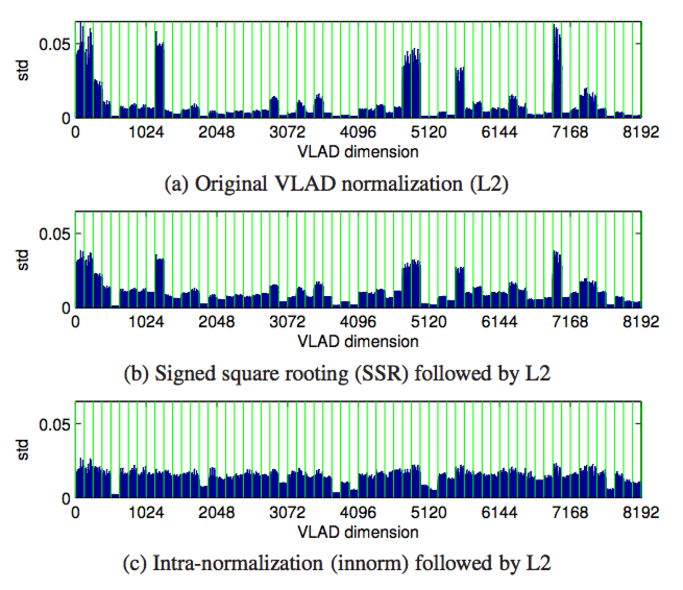
\includegraphics[height=8cm]{figures/vladnorm}
\end{center}
\caption{The effect of normalization on burstiness in VLAD dimension vs. standard deviation (std) which denotes amount of energy stored in that dimension. Clearly intra-normalization followed by L2 normalization evens out energy stored in different VLAD dimensions. Burstiness could result from a repeated structure in the image like a brick wall or a tiled floor for example. \cite{Arandjelovic2013}.}
\label{vladburstiness}
\end{figure}

In \cite{Arandjelovic2013}, Arandjelovi\'{c} and Zisserman modify VLAD in three ways to improve retrieval performance. First they decrease burstiness \cite{Jegou2009}, \cite{Delhumeau2013} (fig. \ref{vladburstiness}), few large components in the VLAD vector can dominate similarity computations. SSR normalization decreases burstiness but does not eliminate it. Intra-normalization alleviates burstiness and improves \emph{mAP} \cite{Arandjelovic2013}. Instead of L2-, or signed square root-normalizing over all descriptor blocks, the sum of the residuals within each VLAD block is normalized. Afterwards L2 normalization is carried out. Intra-normalization is very successful in repressing burstiness (fig. \ref{vladburstiness}).

Second, if the visual vocabulary is trained using one dataset and used on another, the recognition performance suffers. Vocabulary adaptation in \cite{Arandjelovic2013} alleviates the symptoms without re-training the vocabulary, an expensive and inconvenient operation especially for large datasets. It would also require the storing of the original descriptors. \emph{Cluster center adaptation} uses $\hat{\mu}$ which are adapted to the mean of descriptors assigned to the same center $k$. The VLAD descriptors are then updated to use the new centers. Their assignment to a center does not change, but this makes comparing image similarity using VLAD more precise. Vocabulary adaptation and intra-normalization are orthogonal and may be used independently. Increases of as much as 34\% (fig. \ref{vladadapt}) may be observed using both vocabulary adaptation and intra-normalization. \cite{Arandjelovic2013}

\begin{figure}[htb]
\begin{center}
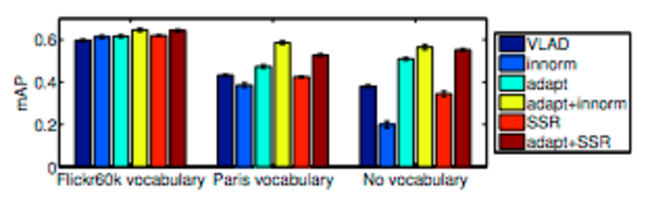
\includegraphics[height=3cm]{figures/vladadapt}
\end{center}
\caption{Comparing retrieval performance in the INRIA Holidays dataset between VLAD, \emph{innorm} intra-normalization, \emph{adapt} vocabulary adaptation, \emph{adapt+innorm} is both vocabulary adaptation and intra-normalization. \cite{Arandjelovic2013}.}
\label{vladadapt}
\end{figure}

Third, VLAD loses to BoW in performance for objects occupying a small portion of the image. \cite{Arandjelovic2013} proposes \emph{Multiple VLAD descriptors} (MultiVLAD), which is especially useful in object recognition. MultiVLAD extracts a total of 14 VLAD descriptors from a single image. A $3 \times 3$ grid over the image gives $9$, $2 \times 2$ grid gives four and one for the whole image. This comes at the cost of memory but is still feasible on off the shelf hardware at ~28GB for 100 million images \cite{Arandjelovic2013}. MultiVLAD outperforms 1792-D (vocab. size) VLAD, but is found to be inferior for images that cover at least 20\% of the image \cite{Arandjelovic2013}.


\clearpage

\section{Materials and methods}
\subsection{Comparing image classifiers}
\subsubsection{Simulated classifier comparison}
\epigraph{Without data you're just another person with an opinion}{W. Edwards Deming}

To compare object instance recognition by SIFT features to perceptual hashing we will run simulations. We are faced with a binary classification problem. Receiver operating characteristics have been useful for visualizing classifier performance \cite{Fawcett2006}. We will construct ROC graphs for the simple hash, dct hash and large scale image retrieval with SIFT features.

To begin production implementation solving the near similar image matching problem with SIFT-features we need to know if the new solution is an improvement over the existing what we call the simple hash and a version DCT hash. A set of images is needed, as well as well as a modified set described in table \ref{modifiedimages} simulating scenarios typically encountered in duplicate image detection.

\def\arraystretch{1.5}
\begin{table}[htb]
\caption{Test image sets and motivations taken from the "Recognition of object instances practical" paintings set of images.}
\label{modifiedimages}
\begin{center}
\begin{tabular}{lp{0.5\linewidth}}
  Modification & Motivation \\
  \hline \hline
  53\% scale& Simulate responsive site case where image has a scaled duplicate. Choose prime percentage to avoid multiple of two to push scaler to produce uneven results.\\
  \hline
  83\% scale& Another scaled case \\
  \hline
  Shave 10px & Simulate cropping image by 10px or removing a border for example\\
  \hline
  10\% border & Adding a border to a known image \\
  \hline
  Rotate 10\% & User corrects the horizon of a photo \\
  \hline
  Normalize histogram & User normalizes the histogram of a photo\\
  \hline
  Saturate colors & User decides to modify the color palette of the image or photo\\
  \hline
  Not in database & Does the system classify images correctly as not in database?\\
\end{tabular}
\end{center}\end{table}

\def\arraystretch{1.5}
\begin{table}[htb]
\caption{True negatives dataset taken from the oxford images in "Recognition of object instances practical".}
\label{truenegatives}
\begin{center}
\begin{tabular}{lp{0.5\linewidth}}
  Modification & Motivation \\
  \hline \hline
  $n$ (true no) images  & Classify images correctly as $N$?\\
\end{tabular}
\end{center}\end{table}

Paintings dataset from the "Recognition of object instances practical" \cite{Vedaldi2012} of a total of 1708 images will be used due to ready scripts for the SIFT case.

An Imagemagick shell script generates manipulated duplicates. 53\% and 83\% scales simulate multiple scales of the same image. Photo straightening is simulated by a 10\% rotation. For color manipulation so we will saturate the image by 50\%. Histogram normalization is quite a common operation, so we will use a normalized version of the image to try to find matches.

To simulate image cropping, we crop from all sides by $10px$. Adding a border is simulated by making duplicates with a 10px border.

To test for images not in the set we will pick 1708 images from the ''Object instance recognition practical'' Oxford dataset and run those images against the paintings set. This will look for a $fp_{rate}$ rate with images that are not in the dataset.

Since we do not know how hamming distance affects classifier performance, we will run all sets for hamming distances 0,4,8 \& 12 to tune the hamming distance.


\subsubsection{Edge cases}
Images smaller than 32px wide or high are ignored by the simple hash and dct hash algorithms. Annotating small images is counterproductive so they are ignored.


\subsection{Near duplicate detection system}

\clearpage

\section{Results}
Modified image sets in tables \ref{modifiedimages} and \ref{truenegatives} were run against all three classifiers, the simple hash, the dct hash and SIFT-classifier. SIFT-classifier outperforms the perceptual hashes in all categories except the simple hash for 53\% scale fig. \ref{tptotal}. The only miss for the SIFT-matcher is a duplicate image in the paintings dataset. SIFT outperforms the perceptual hashes for FP for all test sets in fig. \ref{fptotal}.

For the $TN$ test set the SIFT-classifier performed the worst returning all false positives instead of misses. This was due to not setting a cutoff score. If returned matches from a search score less than this cutoff score, the image should be classified as a $TN$. The max score from the $TN$-set was 19 (fig. \ref{sifttnscores}). In order to determine optimum cutoff, we simulate setting the cutoff score from 1 to 19 and run the simulations for each cutoff score.



\begin{figure}[htb]
\begin{center}
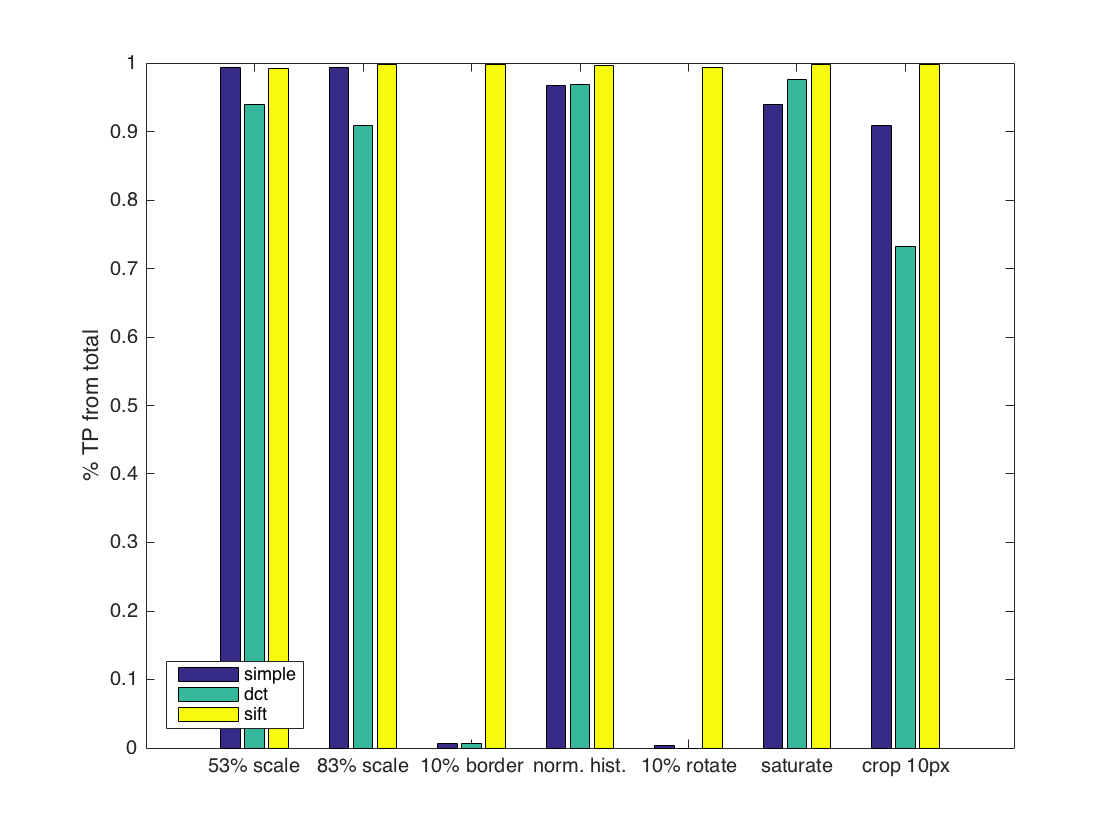
\includegraphics[height=8cm]{figures/tpBar}
\end{center}
\caption{ $TP$ for near duplicate modifications in table \ref{modifiedimages} }
\label{tptotal}
\end{figure}


\begin{figure}[htb]
\begin{center}
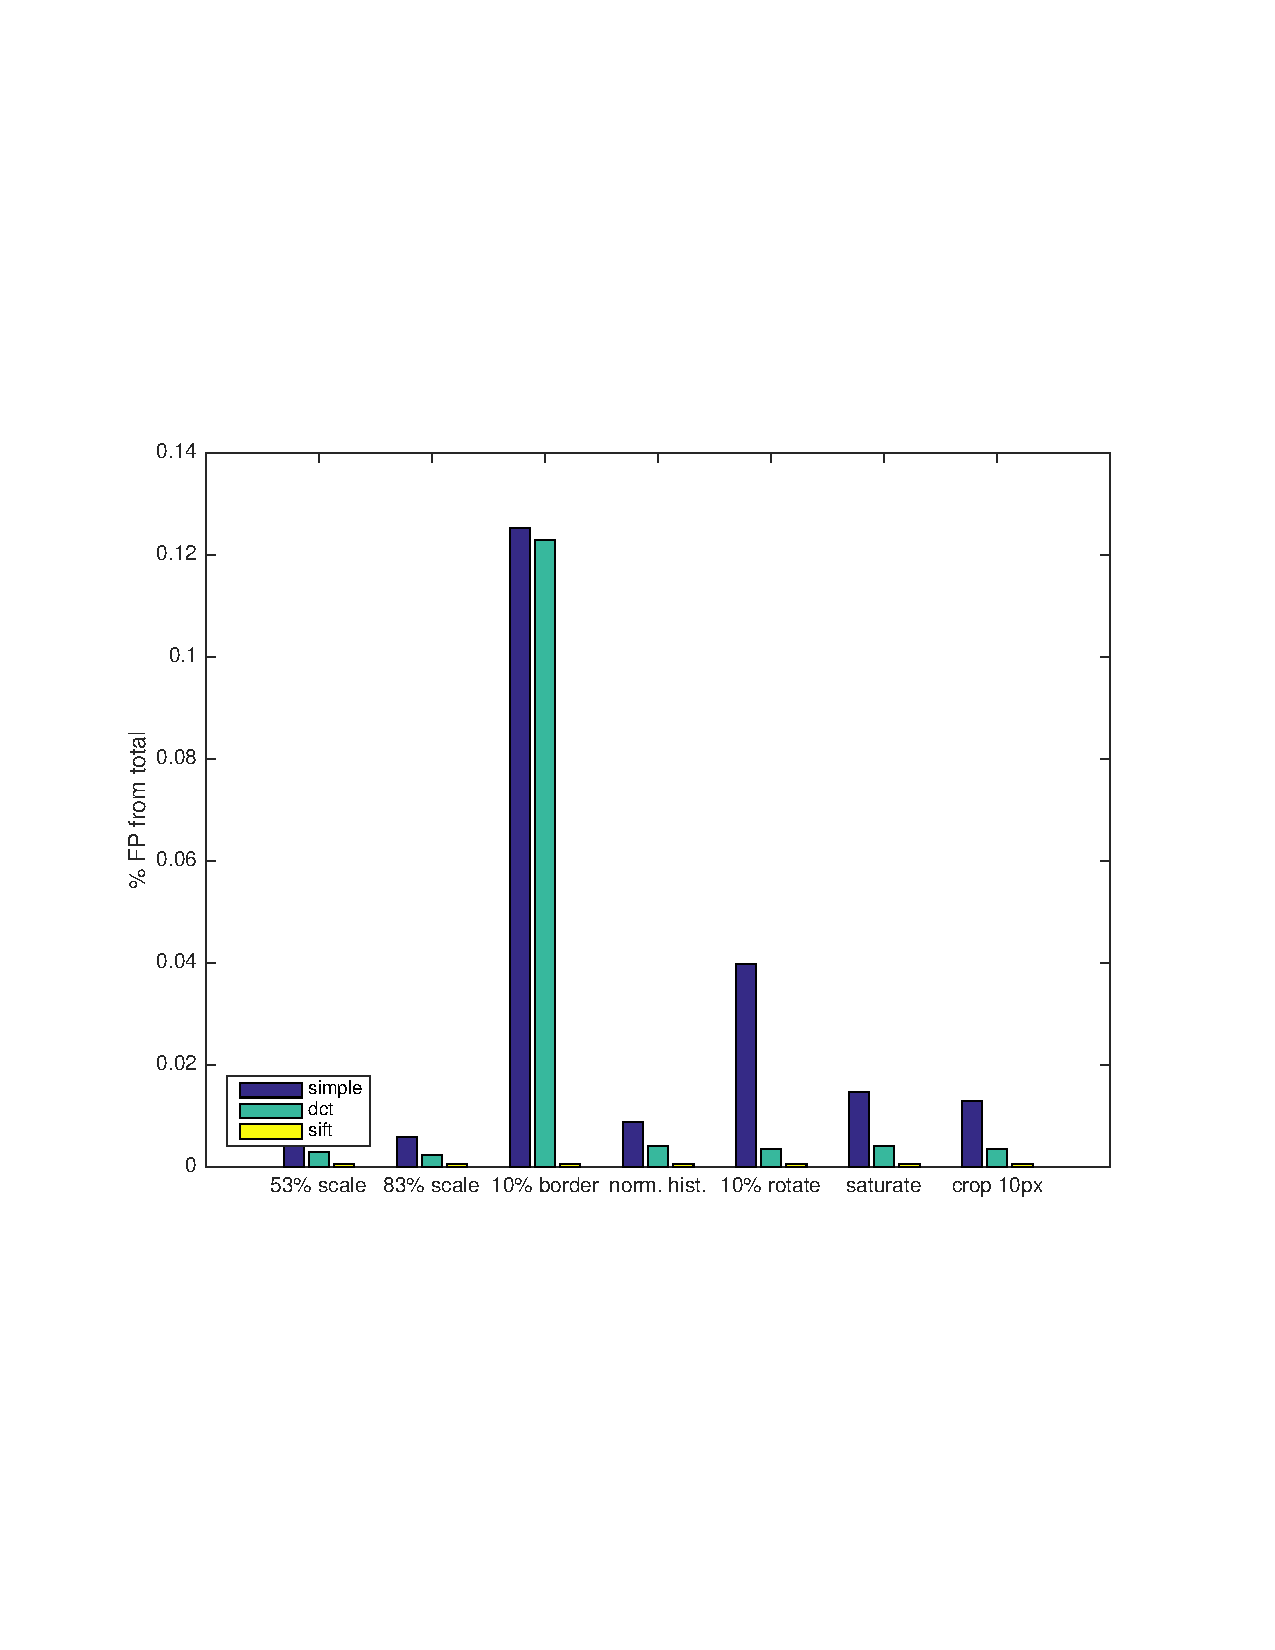
\includegraphics[height=8cm]{figures/fpBar}
\end{center}
\caption{ $FP$ for near duplicate modifications in table \ref{modifiedimages} }
\label{fptotal}
\end{figure}


\begin{figure}[htb]
\begin{center}
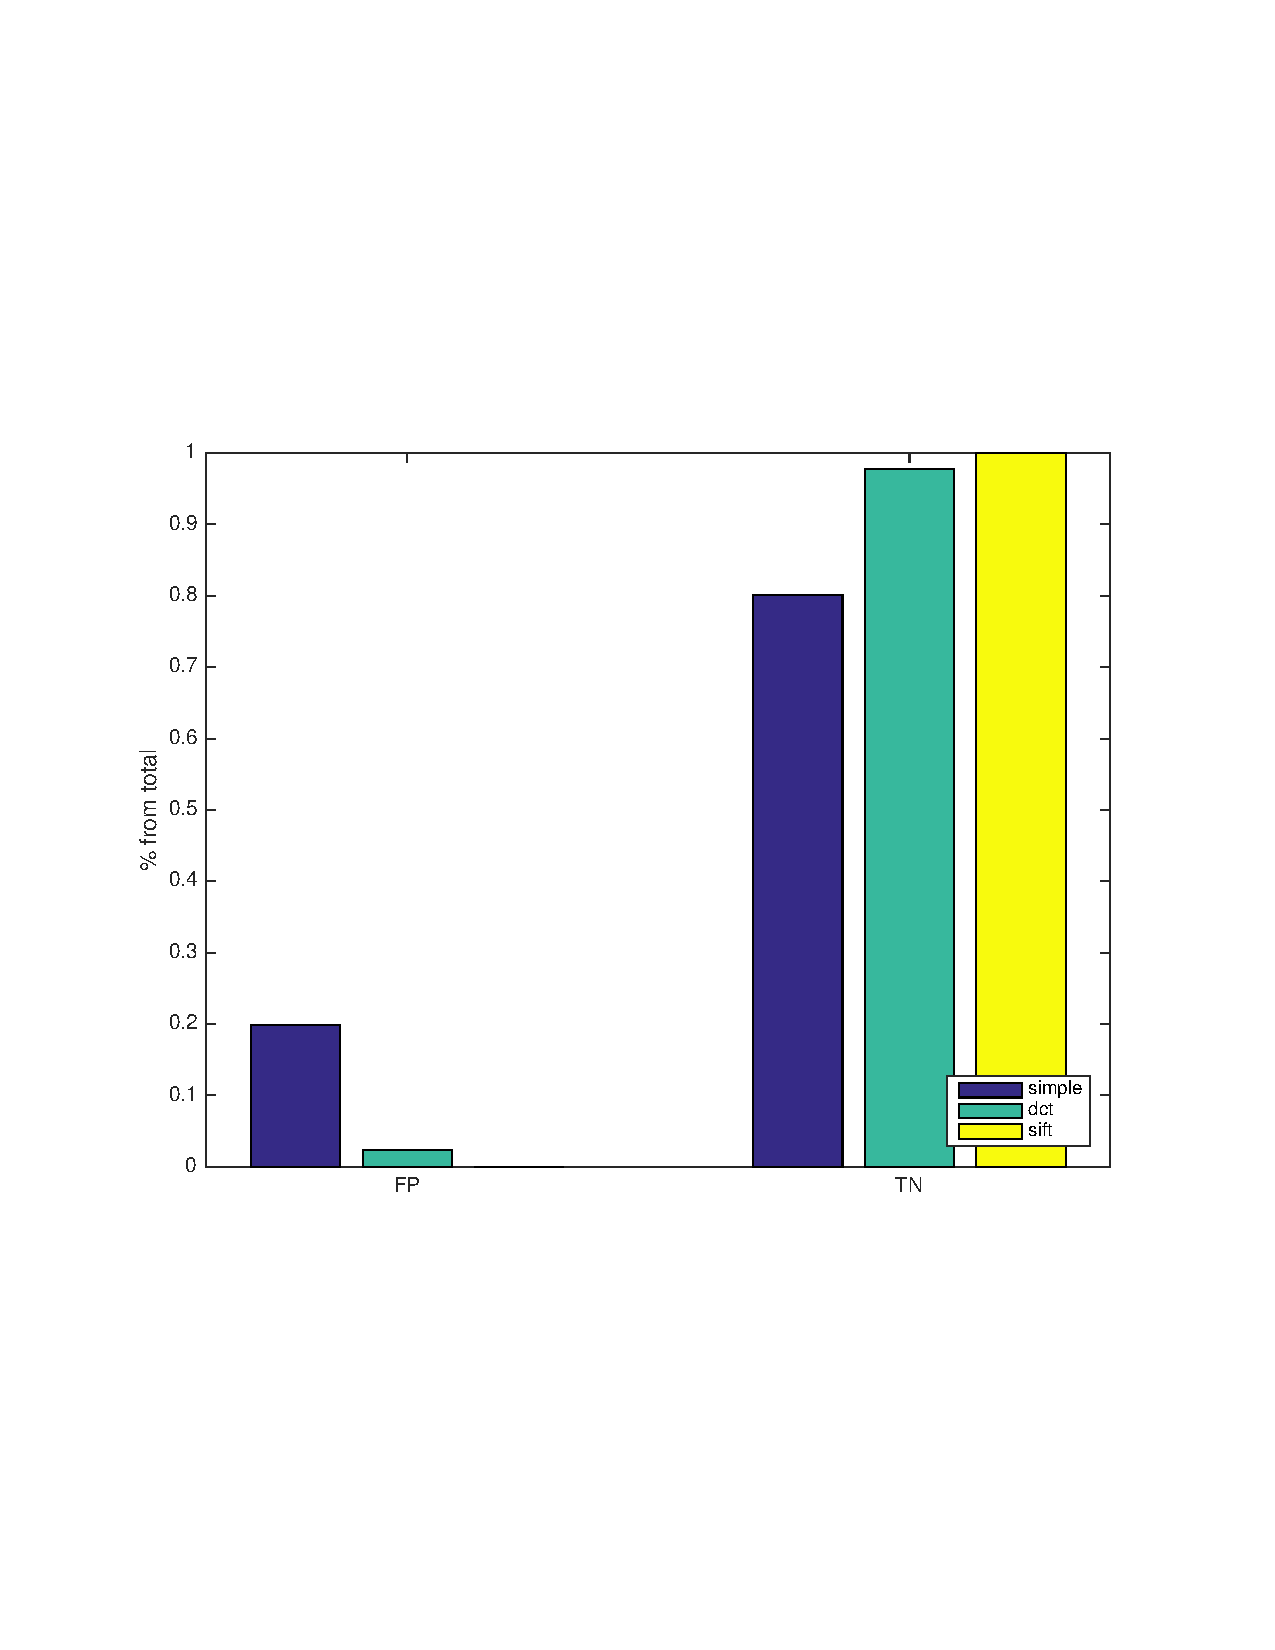
\includegraphics[height=8cm]{figures/tnBar}
\end{center}
\caption{ $TN$ for near duplicate modifications in table \ref{truenegatives} }
\label{tntotal}
\end{figure}

\begin{figure}[htb]
\begin{center}
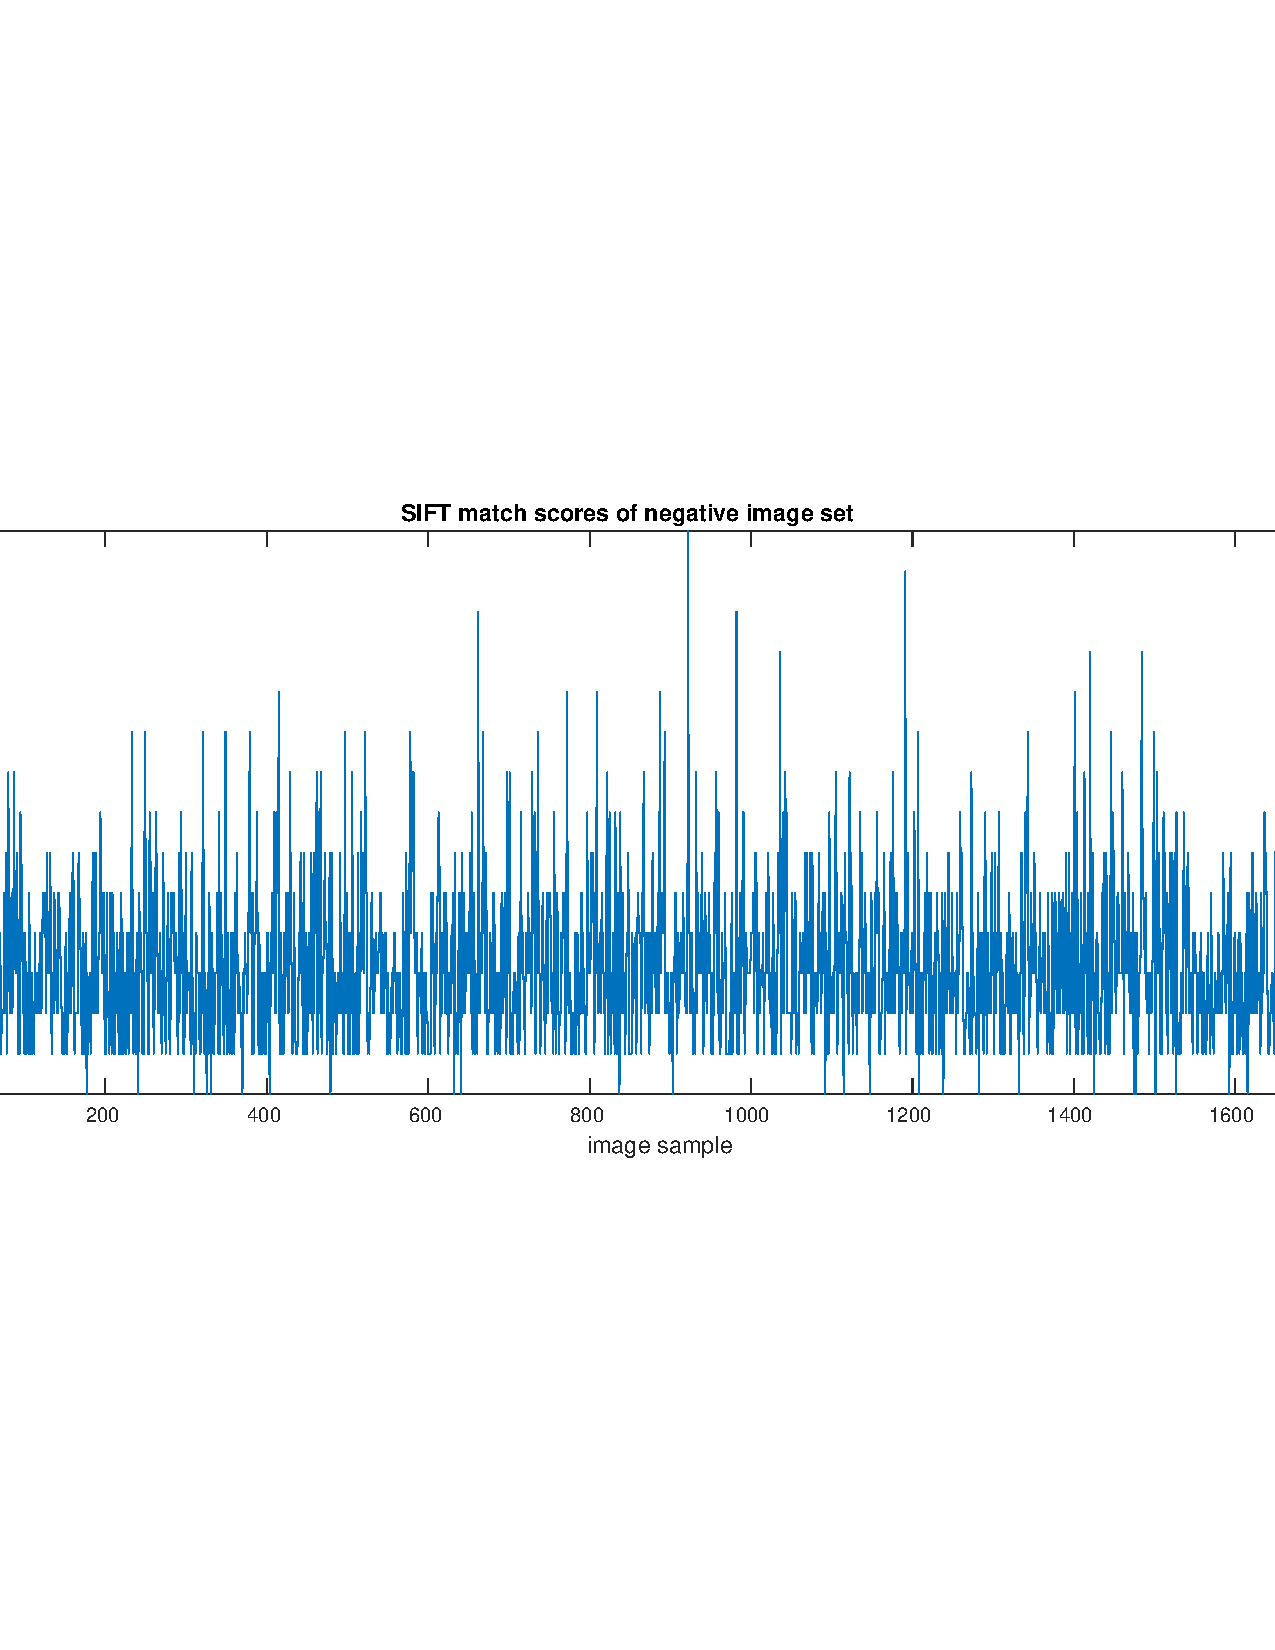
\includegraphics[height=8cm]{figures/cutoff}
\end{center}
\caption{ $TN$ image set max scores returned for images not in database \ref{truenegatives} }
\label{sifttnscores}
\end{figure}




\subsection{Simple hash}

\subsection{DCT Hash}
The $ROC$ of a dct hash based matcher depends on the chosen hamming distance tolerance. The effect on setting hamming distance tolerance on dct hash matcher can be seen in fig. \ref{dcttotalaccuracy}

\begin{figure}[htb]
\begin{center}
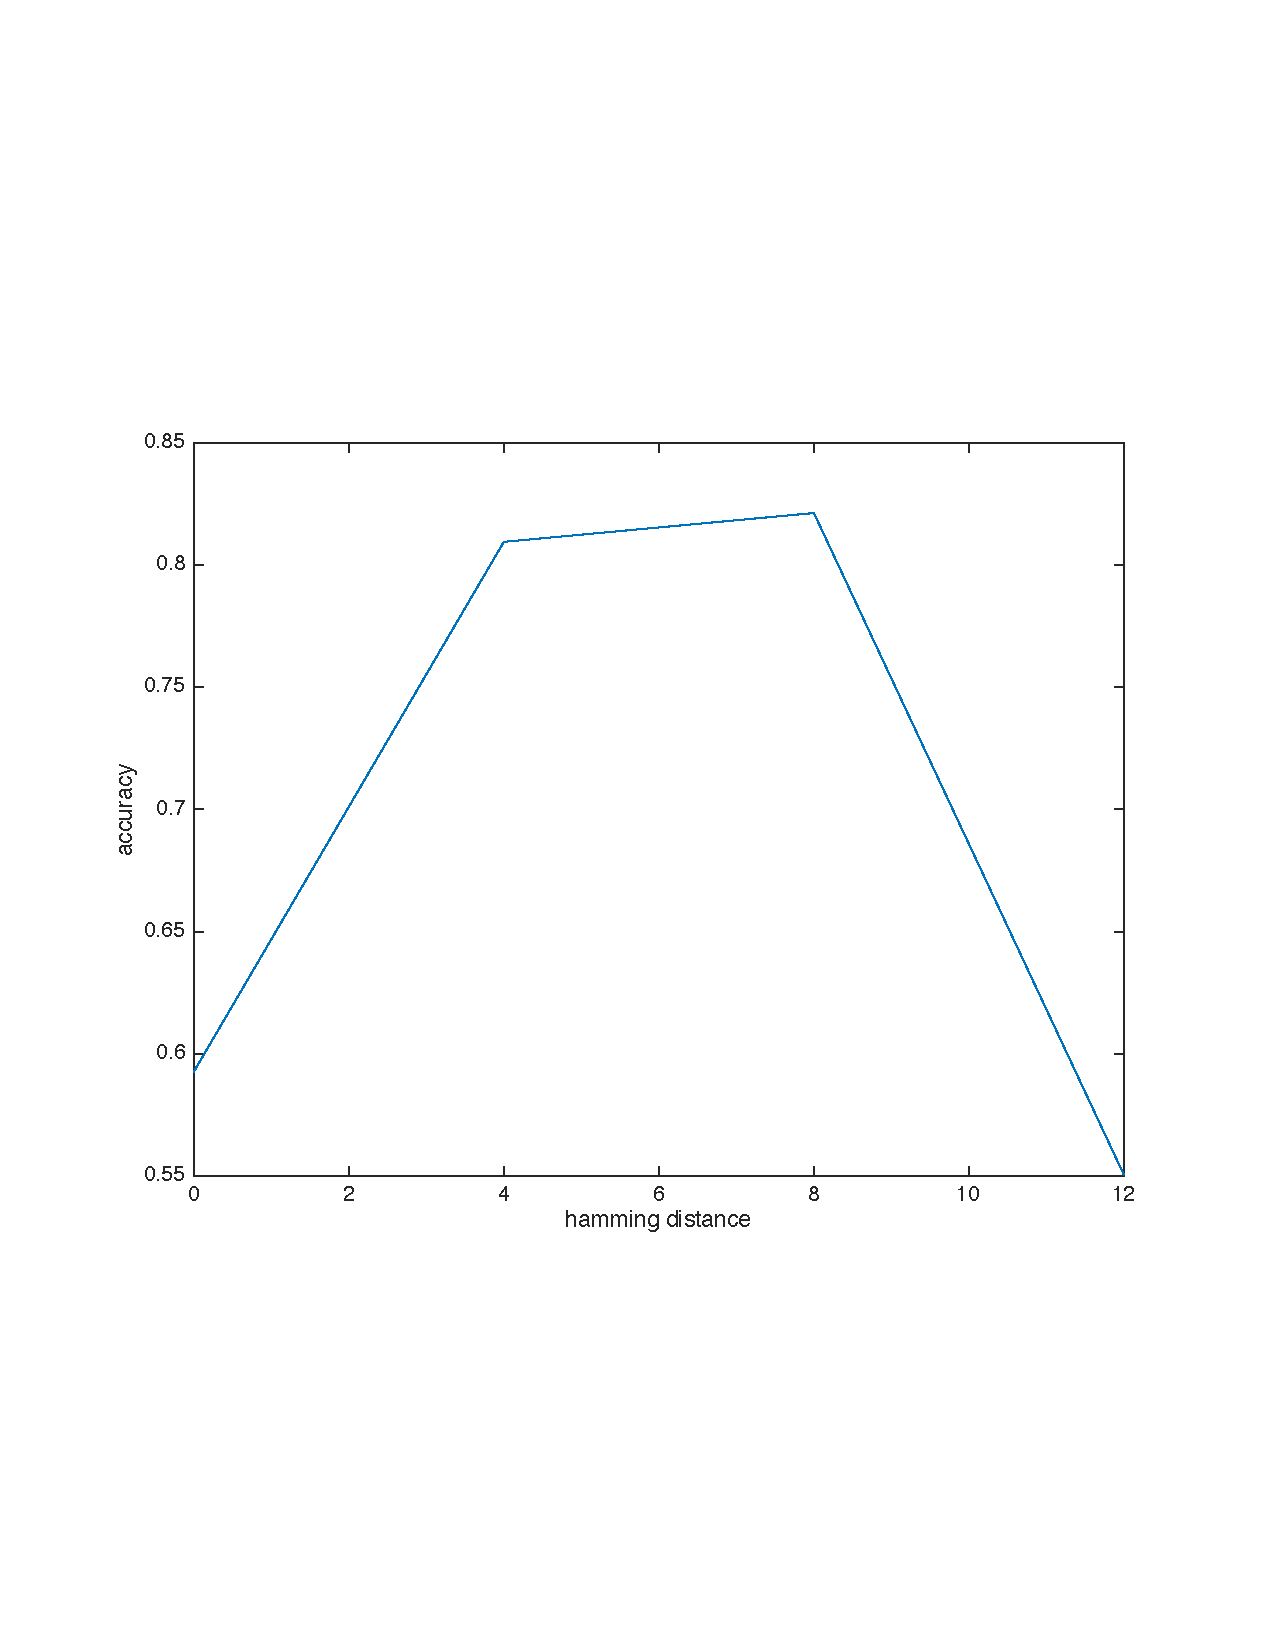
\includegraphics[height=8cm]{figures/dctTotalAccuracy}
\end{center}
\caption{ Effect of Hamming distance tolerance on total accuracy of DCT classifier. }
\label{dcttotalaccuracy}
\end{figure}

\begin{figure}[htb]
\begin{center}
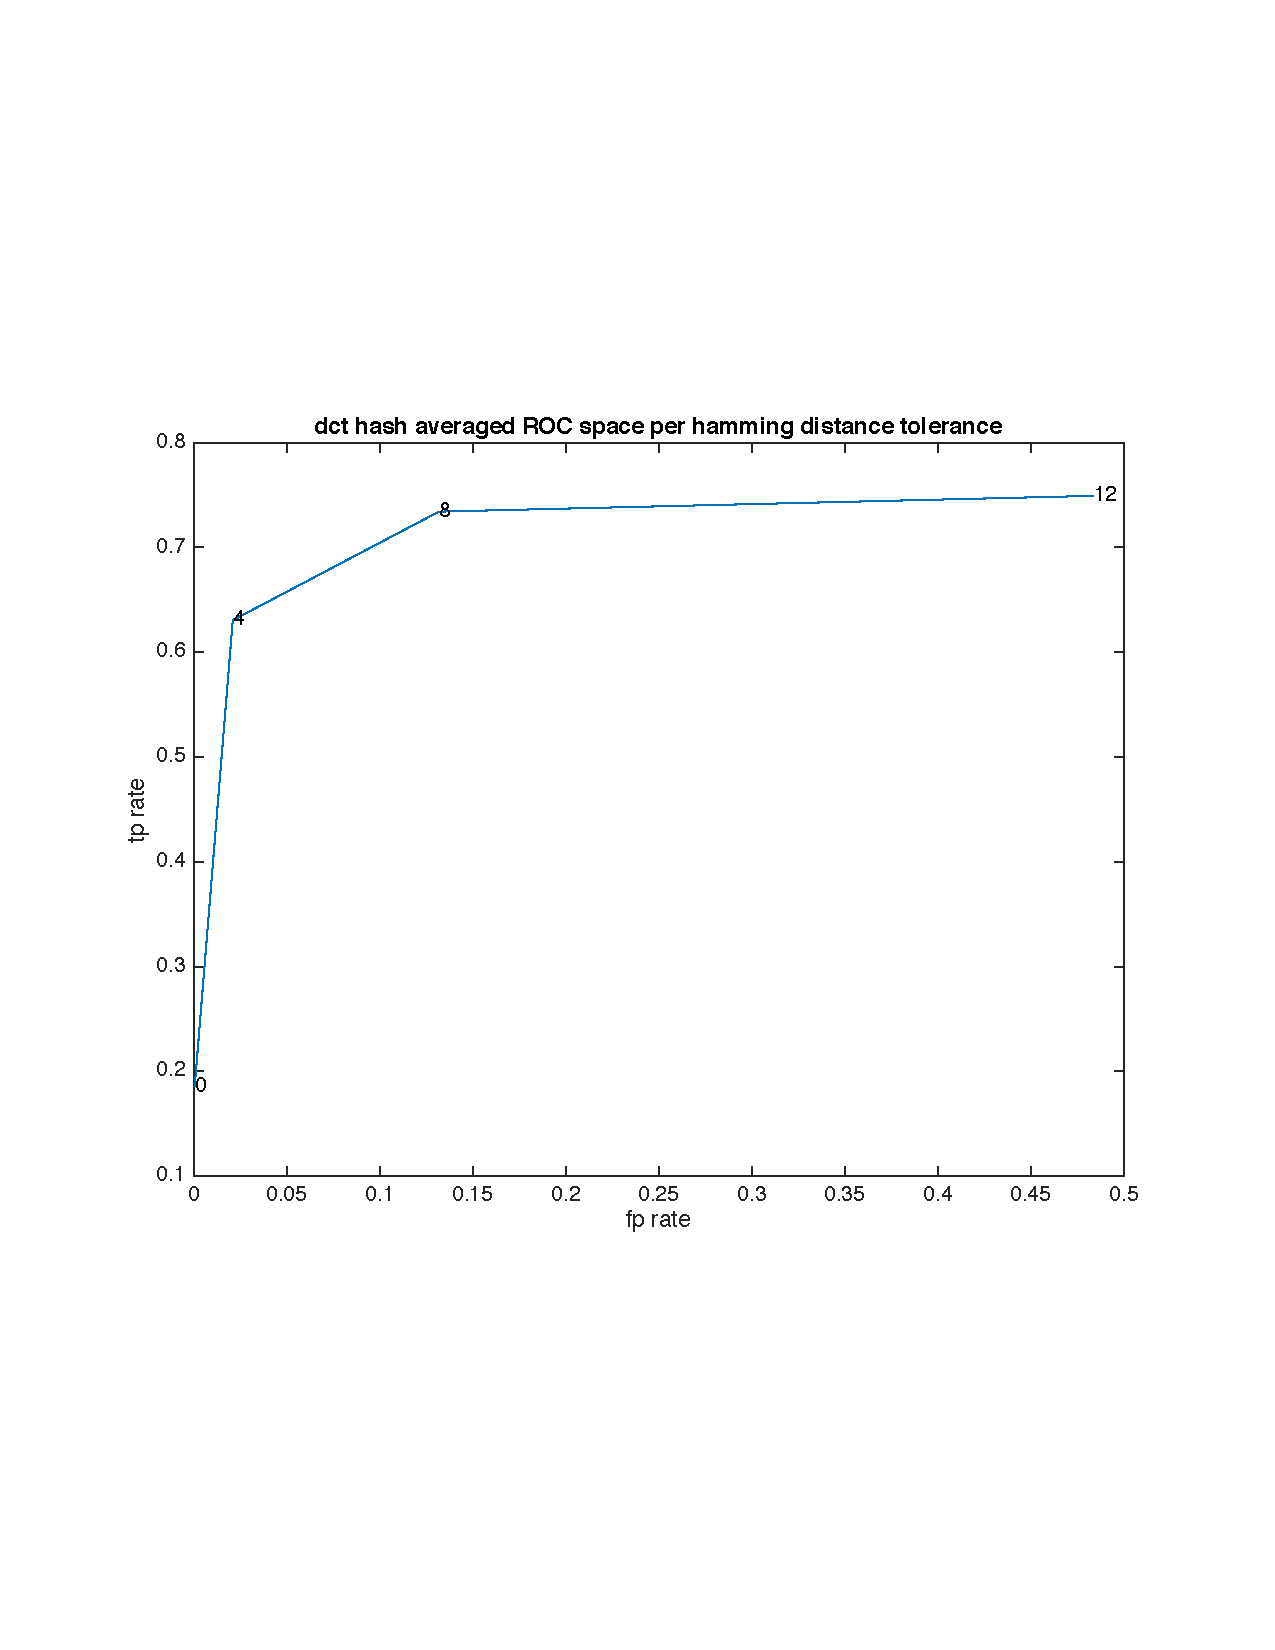
\includegraphics[height=8cm]{figures/dctTotalROC}
\end{center}
\caption{ ROC spamace per hamming distance tolerance based on averaging results on all data. }
\label{dctaverageaccuracy}
\end{figure}


\subsection{Object instance detection by SIFT features}

\subsubsection{Cutoff $C_{s}$}
The search by $SIFT$-features will always return the highest scoring image even if the case of a $fp$. A sane $fp_{rate}$ (close to zero) can be achieved by choosing a cutoff score so that as many as possible of the sets in table \ref{modifiedimages}, and keep true misses to a minimum. We run the sets and plot the scores of matches from each set and find a score such that $tp_{rate}$ is maximized and $fp_{rate}$ is minimized.

Fig. \ref{figcutoffrocspace} shows $SIFT$-classifier performance degrade as $C_{s}->0$. From fig.\ref{figcutoff} we can see the $fn_{count}$ increase linearly as cutoff increases where as the $fp_{count}$ decreases logarithmically as cutoff goes to 19. Plotting the accuracy (eq. \ref{accuracy}) of a the SIFT classifier per $C_{s}$ over data from runs of images in table \ref{modifiedimages} up to

\begin{equation}\label{maxtnscore}
max(score_{tndata}) = 19
\end{equation}

Vertical and horizontal flips are excluded as we do not expect our classifiers to perform well on those. From the test in table \ref{truenegatives}. From fig.\ref{figcutoff} accuracy section we can deduce that the highest accuracy for this data can be achieved by setting $C_{s} = max(score_{tn}) = 19$.

\begin{equation} \label{accuracy}
ACC = \frac{TP +TN}{TP + FP + TN + FN}
\end{equation}

\begin{figure}[htb]
\begin{center}
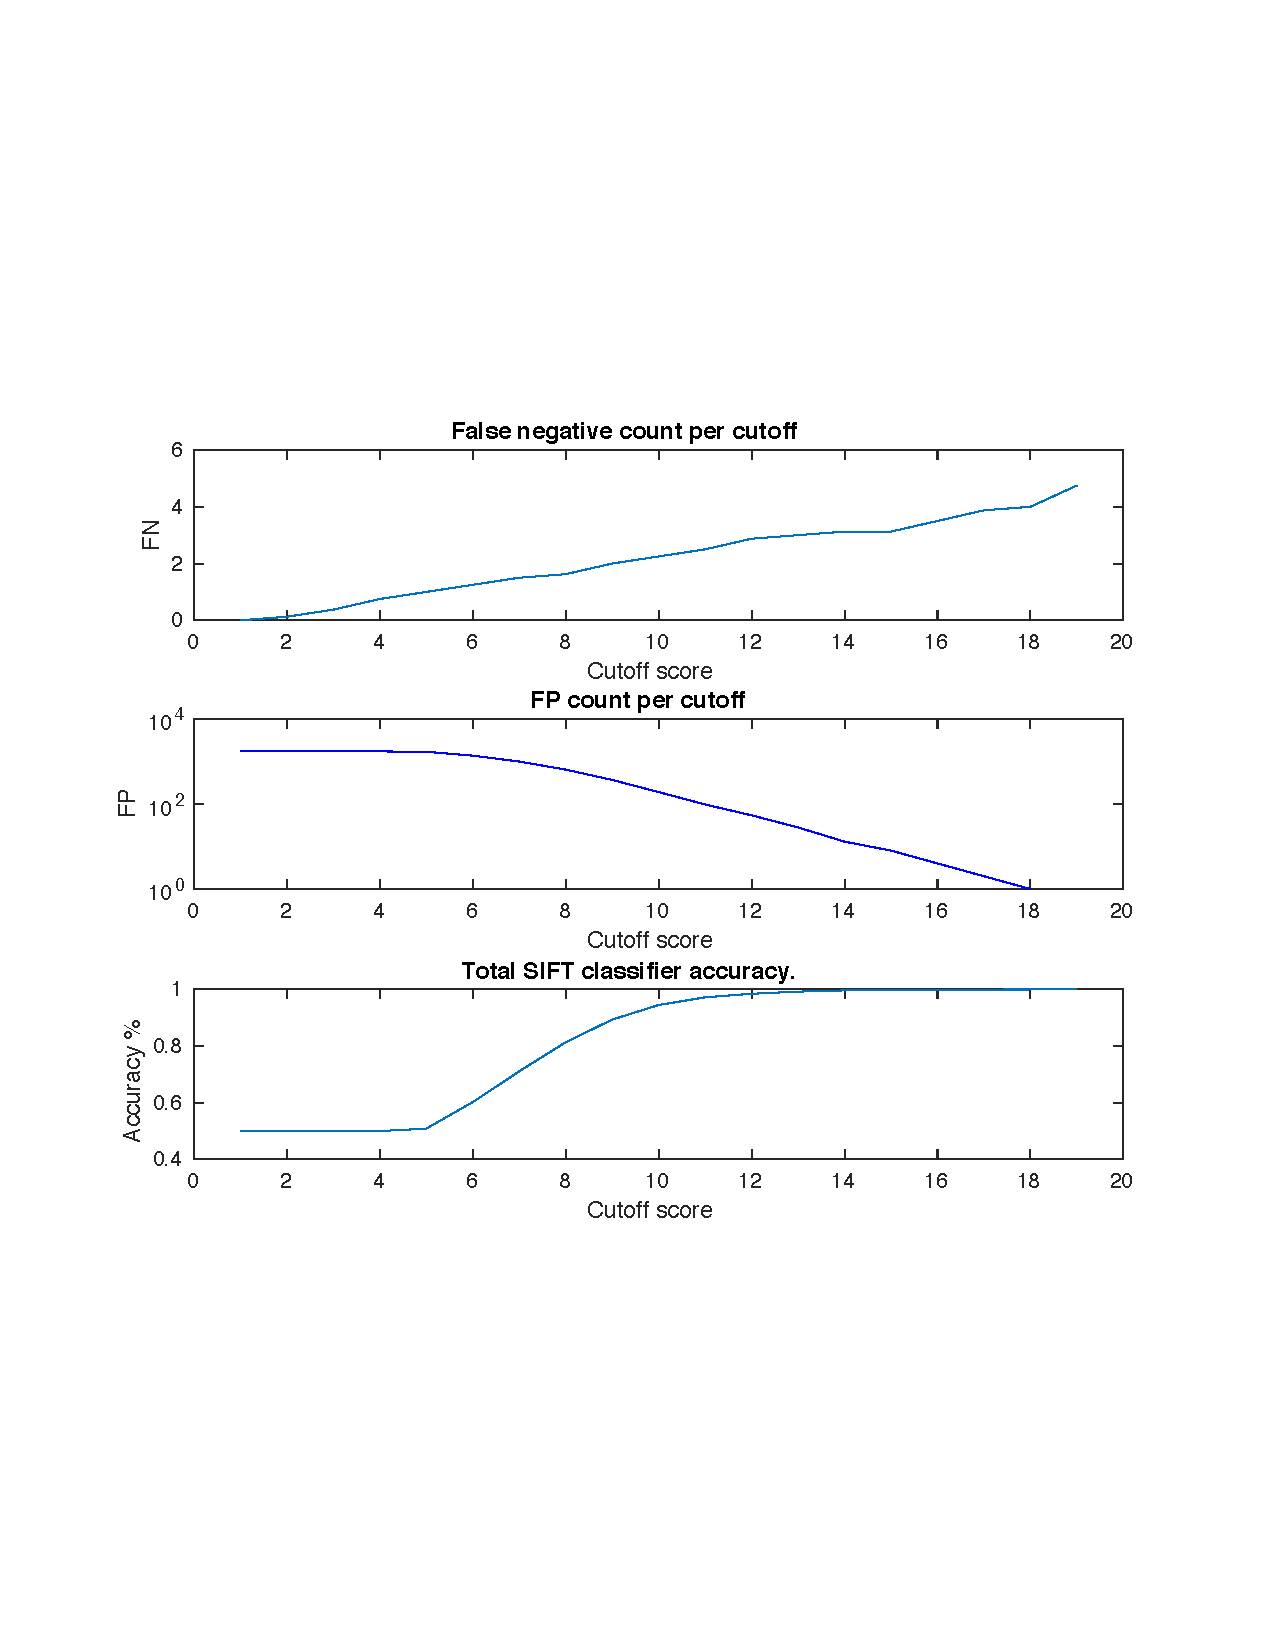
\includegraphics[height=8cm]{figures/SIFTCountROC}
\end{center}
\caption{ Effects of cutoff on SIFT performance. }
\label{figcutoff}
\end{figure}

\begin{figure}[htb]
\begin{center}
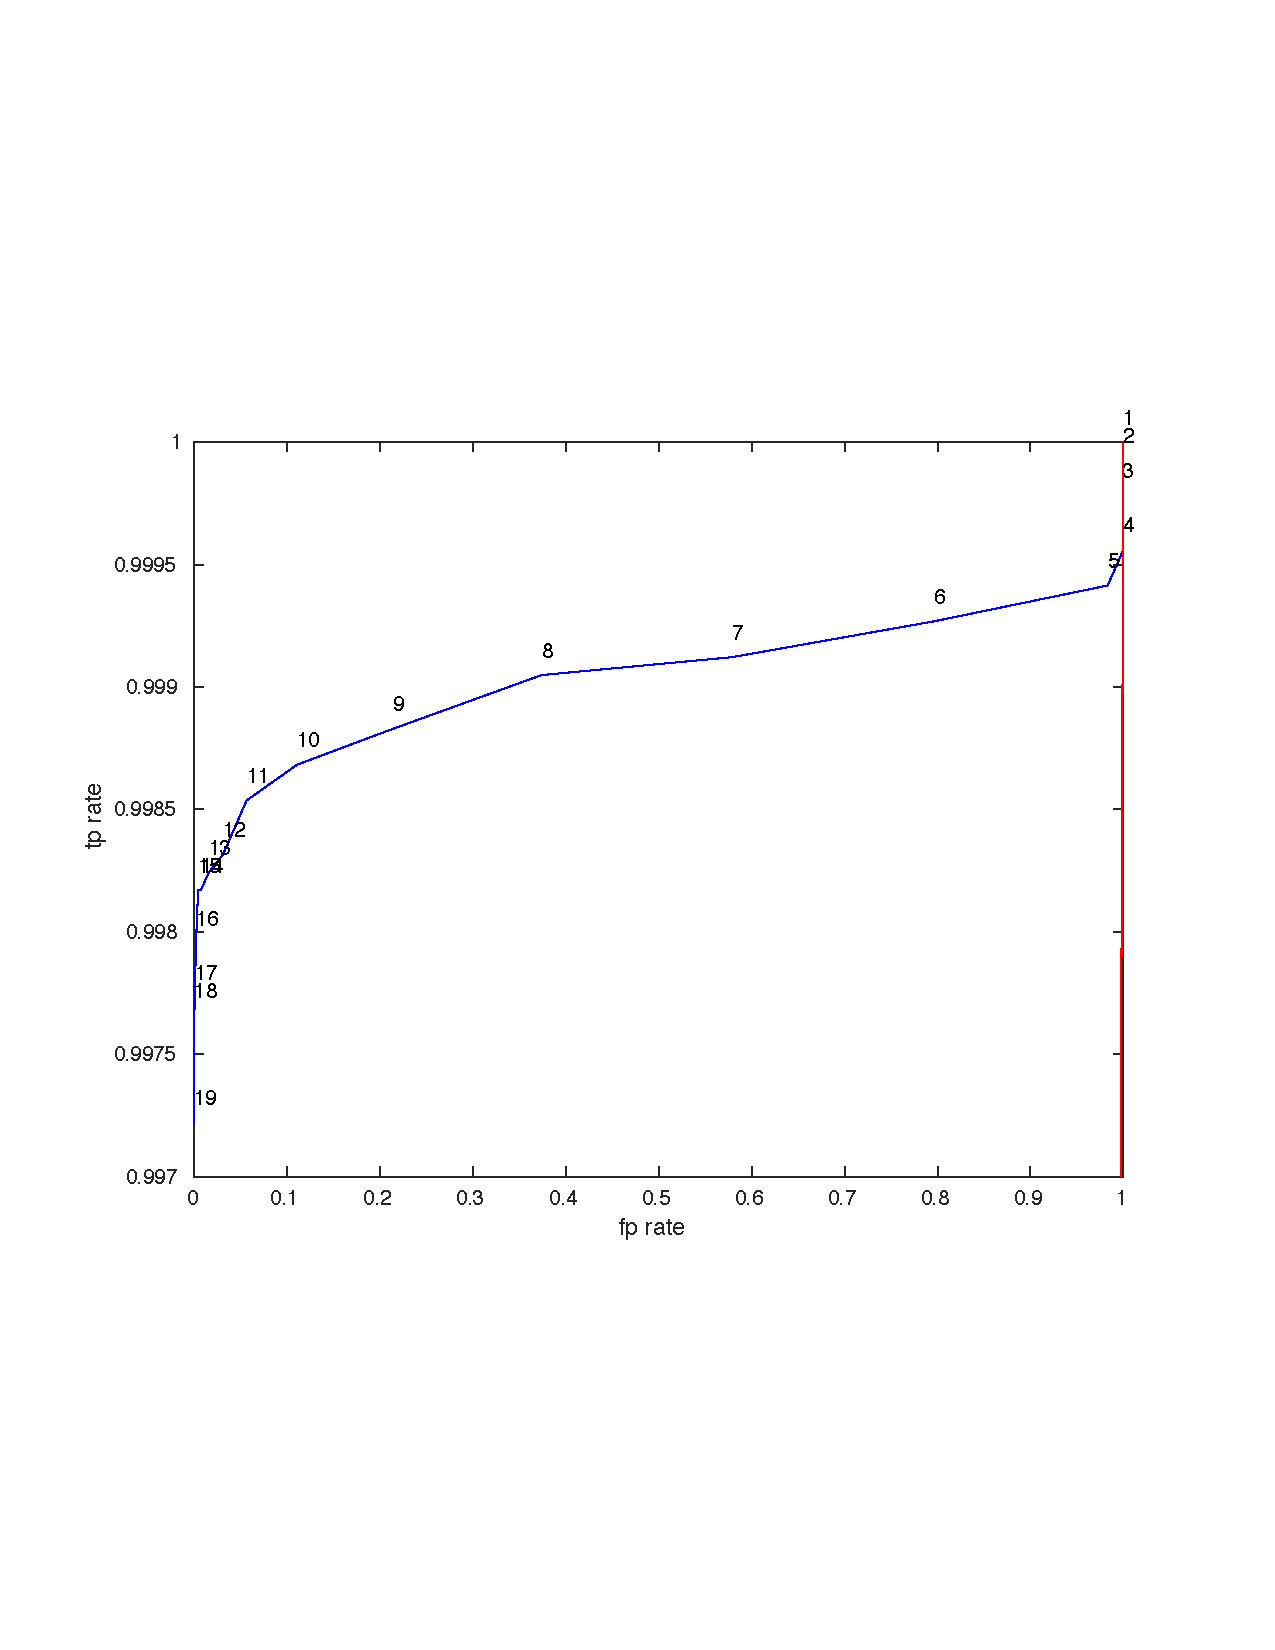
\includegraphics[height=8cm]{figures/SIFTROCperCutoff}
\end{center}
\caption{ ROC Space per SIFT classifier cutoff. }
\label{figcutoffrocspace}
\end{figure}



\subsection{Simulated classifier comparison}
All classifiers in ROC space.

The optimum hamming distance for the classifier using simple hash seems to be 4.
The optimum hamming distance to use with a dct hash classifier seems to be 4.

A table of all the tp and fp rates.
A table with all the numbers from the ROC section.

Put all classifiers in ROC space for all cases.

roc graph over all cases in small multiples

\subsection{System for near duplicate detection by local features}


\clearpage

\section{Discussion}
Any conclusions from the ROC graphs. What recommendation to make? What to take a look at.



\clearpage
%% L\"ahdeluettelo
%%
%% \phantomsection varmistaa, ett\"a hyperref-paketti latoo hypertekstilinkit
%% oikein.
%%
%% The \phantomsection command is nessesary for hyperref to jump to the
%% correct page, in other words it puts a hyper marker on the page.

\phantomsection
\addcontentsline{toc}{section}{\refname}
%\addcontentsline{toc}{section}{References}
\bibliographystyle{plain}
\bibliography{sources}{}

%% Appendices
%% Liitteet
\clearpage

\thesisappendix

\section{Esimerkki liitteest\"a\label{LiiteA}}

Liitteet eiv\"at ole opinn\"aytteen kannalta v\"altt\"am\"att\"omi\"a ja
opinn\"aytteen tekij\"an on
kirjoittamaan ryhtyess\"a\"an hyv\"a ajatella p\"arj\"a\"av\"ans\"a ilman liitteit\"a.
Kokemattomat kirjoittajat, jotka ovat huolissaan
tekstiosan pituudesta, paisuttavat turhan
helposti liitteit\"a pit\"a\"akseen tekstiosan pituuden annetuissa rajoissa.
T\"all\"a tavalla ei synny hyv\"a\"a opinn\"aytett\"a.

Liite on itsen\"ainen kokonaisuus, vaikka se t\"aydent\"a\"akin tekstiosaa.
Liite ei siten ole pelkk\"a listaus, kuva tai taulukko, vaan
liitteess\"a selitet\"a\"an aina sis\"all\"on laatu ja tarkoitus.

Liitteeseen voi laittaa esimerkiksi listauksia. Alla on
listausesimerkki t\"am\"an liitteen luomisesta.

%% Verbatim-ymp\"arist\"o ei muotoile tai tavuta teksti\"a. Fontti on monospace.
%% Verbatim-ymp\"arist\"on sis\"all\"a annettuja komentoja ei LaTeX k\"asittele.
%% Vasta \end{verbatim}-komennon j\"alkeen jatketaan k\"asittely\"a.
\begin{verbatim}
	\clearpage
	\appendix
	\addcontentsline{toc}{section}{Liite A}
	\section*{Liite A}
	...
	\thispagestyle{empty}
	...
	teksti\"a
	...
	\clearpage
\end{verbatim}

Kaavojen numerointi muodostaa liitteiss\"a oman kokonaisuutensa:
\begin{eqnarray}
d \wedge A  &=& F, \label{liitekaava1}\\
d \wedge F  &=& 0. \label{liitekaava2}
\end{eqnarray}


\clearpage
\section{Toinen esimerkki liitteest\"a\label{LiiteB}}

%% Liitteiden kaavat, taulukot ja kuvat numeroidaan omana kokonaisuutenaan
%%
%% Equations, tables and figures have their own numbering in Appendices
%\renewcommand{\theequation}{B\arabic{equation}}
%\setcounter{equation}{0}
%\renewcommand{\thefigure}{B\arabic{figure}}
%\setcounter{figure}{0}
%\renewcommand{\thetable}{B\arabic{table}}
%\setcounter{table}{0}

Liitteiss\"a voi my\"os olla kuvia, jotka
eiv\"at sovi leip\"atekstin joukkoon:
%% Ymp\"arist\"on figure parametrit htb pakottavat
%% kuvan t\"ah\"an, eik\"a LaTeX yrit\"a siirrell\"a niit\"a
%% hyv\"aksi katsomaansa paikkaan.
%% Ymp\"arist\"o\"a center voi k\"aytt\"a\"a \centering-
%% komennon sijaan
%%
%% Example of a figure, note the use of htb parameters which force
%% the figure to be inserted here
\begin{figure}[htb]
\begin{center}
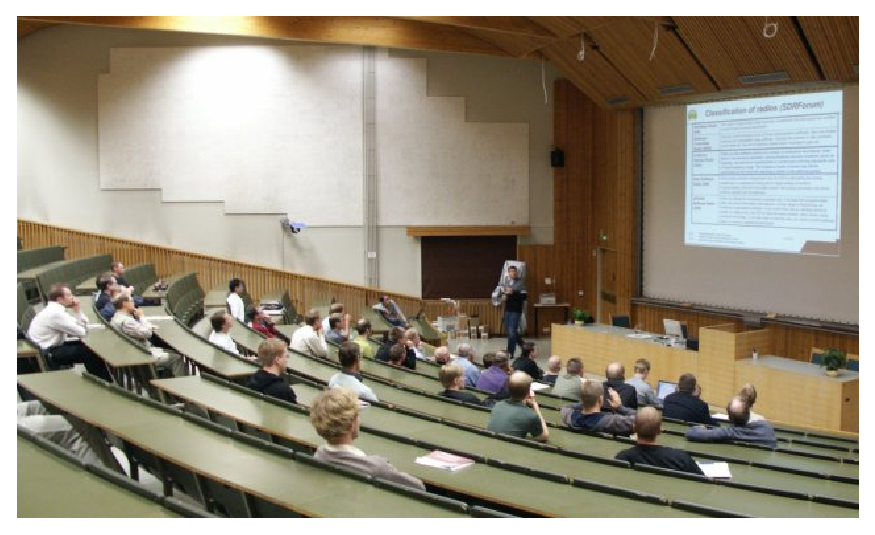
\includegraphics[height=8cm]{kuva2}
\end{center}
\caption{Kuvateksti, jossa on liitteen numerointi}
\label{liitekuva}
\end{figure}
%%
Liitteiden taulukoiden numerointi on kuvien ja kaavojen kaltainen:
\begin{table}[htb]
\caption{Taulukon kuvateksti.}
\label{liitetaulukko}
\begin{center}
\fbox{
\begin{tabular}{lp{0.5\linewidth}}
9.00--9.55  & K\"aytett\"avyystestauksen tiedotustilaisuus (osanottajat
ovat saaneet s\"ahk\"opostitse valmistautumisteht\"av\"at, joten tiedotustilaisuus
voidaan pit\"a\"a lyhyen\"a).\\
9.55--10.00 & Testausalueelle siirtyminen
\end{tabular}}
\end{center}
\end{table}
Kaavojen numerointi muodostaa liitteiss\"a oman kokonaisuutensa:
\begin{eqnarray}
T_{ik} &=& -p g_{ik} + w u_i u_k + \tau_{ik},  \label{liitekaava3} \\
n_i    &=& n u_i + v_i.                      \label{liitekaava4}
\end{eqnarray}

\end{document}
